\documentclass[a4paper, twoside, 12pt]{book}

\usepackage{fontspec}
\usepackage[greek,french]{babel}
%--------------------------
% INPUTENC (encodage du texte)
% FONTENC (positionnement des accents)
%--------------------------
\usepackage[utf8]{inputenc}
%\usepackage{ae,lmodern}
\usepackage[T1]{fontenc}
\usepackage{minted}

\usepackage{subcaption}
\usepackage{caption}

% Interligne
\usepackage{setspace}

%Pour gérer caractères spéciaux °
%\DeclareUnicodeCharacter{00B0}{ }

%Pour les épigraphes
\usepackage{epigraph}
\setlength{\epigraphrule}{0pt}
\setlength{\epigraphwidth}{0.6\textwidth}
\renewcommand\textflush{flushepinormal}
\renewenvironment{flushepinormal}{}{\vspace*{-\baselineskip}}


%--------------------------
% HYPERREF (liens hypertextes et métadonnées)
%--------------------------
\usepackage{hyperref}
\hypersetup{%
colorlinks=true,
linkcolor=black,
urlcolor=blue,
citecolor=black
}

%--------------------------
% TOCBIBIND (ajouter la bibliographie dans la Table des matières)
%--------------------------
\usepackage{tocbibind}
%--------------------------
% Éléments de mise en page (marge de 2,5 cm, alinéa en début de paragraphe 1cm, interligne 1,5)
%--------------------------
\usepackage[a4paper, margin=2.5cm]{geometry}
\usepackage{setspace}
\onehalfspacing
\setlength{\parindent}{1cm}

\usepackage{fancyhdr}
\setlength{\headheight}{28pt}
\renewcommand{\chaptermark}[1]{\markboth{#1}{}}
\renewcommand{\sectionmark}[1]{\markright{#1}}
\pagestyle{fancy}
\fancyhf{}
\fancyhead[LE,RO]{\thepage}
\fancyhead[LO]{\nouppercase{\rightmark}}
\fancyhead[RE]{\nouppercase{\leftmark}}
\renewcommand{\headrulewidth}{0pt}

%--------------------------
% Modules pour gérer les listes
%--------------------------
\usepackage{enumerate}
\usepackage{enumitem}

%use special characters unicode
\usepackage{xunicode}
\setmainfont[Numbers=OldStyle]{Junicode}
\defaultfontfeatures{Ligatures=TeX}
\usepackage{xspace}

%--------------------------
% BIBLIOGRAPHIE
%--------------------------
\usepackage[backend=biber, sorting=nyt, style=enc]{biblatex}
\usepackage[autostyle]{csquotes}

%\bibliography{mybibliography.bib}
\addbibresource{biblio_temp_tech.bib}


\setcounter{secnumdepth}{5}
\setcounter{tocdepth}{2}

\usepackage[official]{eurosym}
\usepackage{afterpage}

%--------------------------
% FIGURES
%--------------------------
\usepackage{graphicx}
\graphicspath{ {./images/} }
\usepackage{float}
% ============================================

\begin{document}

\frontmatter
\include{front/titlepage}
\include{front/abstract}

\begin{titlepage}
\begin{center}

\bigskip

\begin{large}
UNIVERSITÉ PARIS, SCIENCES \& LETTRES
\end{large}

\begin{center}\rule{2cm}{0.02cm}\end{center}

\bigskip
\bigskip
\bigskip
\begin{Large}
\textbf{Malamatenia Vlachou-Efstathiou}\\
\end{Large}
\begin{normalsize}
\textit{Diplômée de Licence en Lettres Classiques}\\
\textit{Diplômée de Master en Latin}\\
\end{normalsize}

\bigskip
\bigskip
\bigskip

\begin{Huge}
\textbf{Éditer les manuscrits grammaticaux glosés : solutions numériques face aux défis traditionnels}\\
\end{Huge}

\bigskip
\bigskip
\begin{LARGE}
\textbf{Le cas du \textit{Voss.Lat.}O.41 d'Eutychès}\\
\end{LARGE}

\bigskip
\bigskip
\bigskip
\vfill

\begin{large}
Mémoire de première année du master\\
\og Humanités Numériques \fg{} \\
\bigskip
juin 2022
\end{large}

\end{center}
\end{titlepage}

\section*{Résumé}
\addcontentsline{toc}{chapter}{Résumé}
En règle générale, les manuscrits grammaticaux glosés constituent un défi pour les chercheurs qui souhaitent les éditer. Leur caractère hétérogène reflété dans les spécificités structurelles de leur \textit{mise-en-page}, ainsi que dans les multiples couches d'annotations et de variations orthographiques, font de leur modélisation une tâche difficile. Les outils numériques, comme en témoignent des projets récents, offrent une variété de solutions qui se révèlent particulièrement efficaces et donc nécessaires pour leur édition, du HTR et les vocabulaires contrôlés jusqu'au XML-TEI et la visualisation des données.En prenant le \textit{Vossianus Latinus} O41 du \textit{de uerbo} d'Eutyches comme cas d'étude, nous tâcherons de mettre en œuvre un pipeline semi-automatique vers une édition documentaire multifonctionnelle.

\medskip

\textbf{Mots-clés: paléographie latine ; Grammatici Latini ; maniscrits glosés ; Eutychès; humanités numériques ; HTR ; apprentissage machine; ALTO; XSL; SegmOnto ; XML-TEI }

\textbf{Informations bibliographiques:} Malamatenia Vlachou-Efstathiou, \textit{Éditer les manuscrits grammaticaux glosés : solutions numériques face aux défis traditionnels : Le cas du \textit{Voss.Lat. O.41} d'Eutychès}, mémoire de master 1 \og Humanités Numériques\fg{}, dir. [Cécile Conduché, Peter A. Stokes], Université Paris, Sciences \& Lettres, 2022.


\section*{Abstract}
\addcontentsline{toc}{chapter}{Abstract}
Generally, glossed grammatical manuscripts pose a significant challenge to researchers that wish to edit them. Their heterogenous character reflected in the structural specificities of their \textit{mise-en-page}, alongside often multiple layers of annotations and orthographical variation, make their modeling a difficult task. Digital tools, as recent projects attest, offer a variety of solutions that reveal particularly efficient and thus necessary for their edition, from HTR and controled vocabularies to XML-TEI and the visualisation of the data. With Eutyches' \textit{Vossianus Latinus} O41 of the \textit{de uerbo} as a case study, we'll try to apply a semi-automatised pipeline towards a multifunctional documentary edition.

\medskip

\textbf{Keywords: latin paleography ; Grammatici Latini  ; glossed manuscripts ; Eutyches digital humanities ; HTR  : machine learning; ALTO; XSL; SegmOnto ; XML-TEI }

\textbf{Bibliographic Information:}, Malamatenia Vlachou-Efstathiou \textit{Editing glossed grammatical manuscripts : digital solutions to traditional challenges : The case of the \textit{Voss.Lat. O.41} of Eutyches}, mémoire de master 1 \og Humanités Numériques\fg{}, dir. [Cécile Conduché, Peter A. Stokes], Université Paris, Sciences \& Lettres, 2022.

\clearpage

\section*{Remercîments}

Avant la présentation du projet, je tiens à remercier brièvement tous ceux qui ont contribué à l'élaboration de ce mémoire, à quelque étape et de quelque façon que ce soit. Leur aide s'est révélée extrêmement précieuse tout au long de cette année, alors que je me lançais progressivement dans le domaine des Humanités Numériques.\\

Tout d'abord, je voudrais remercier mes deux directeurs de recherche. D’une part Mme Cécile Conduché, qui m'a fait découvrir l'œuvre d'Eutychès et ses défis, a partagé avec moi son travail et a fait confiance à mes capacités face à un manuscrit inédit. De l’autre Mr. Peter Stokes, qui a accepté de m'encadrer et qui a été patient dès le début alors que je me familiarisais lentement avec les spécificités de mon jeu de données et toutes les possibilités que le numérique avait à offrir à ma recherche. Sur le même plan, je remercie chaleureusement Mme Cécile Lanéry de l'IRHT qui m'a appris tout ce que je connais sur la paléographie latine et dont la passion pour cette discipline je partage et j’admire. \\

 En même temps, je suis très reconnaissante aux professeurs de l'ENC qui ont bien voulu m'accompagner dans mon travail et qui ont pris le temps, dans les moments de détresse, d'écouter patiemment mes problèmes et mes idées et de m'aider à trouver des solutions. Je me réfère plus particulièrement à Mr. Thibault Clérice, Mme Lucence Ing et Mr.Chahan Vidal-Gorène sans l'orientation desquels ce projet n'aurait pas été le même.Un sincère merci va également à l'équipe de \textit{Gallicorpora}, Mme Ariane Pinche, Mr. Simon Gabay, et mes collègues, avec qui j'ai eu la chance de travailler et d'apprendre, notamment de m'avoir fait découvrir le potentiel d'eScriptorium et de Segmonto. \\

Je voudrais remercier aussi mes camarades et amis, d’avoir partagé avec moi cette année académique intense, de m'avoir fait me sentir la bienvenue malgré mon origine étrangère, et de m'avoir fait part de leurs propres projets, passions et connaissances. Sans eux, tout ce processus n'aurait pas été aussi agréable et constructif. Enfin, un énorme merci à mon père et à ma sœur qui m'ont toujours soutenue quoi qu'il arrive, et ont cru en moi quand je ne le faisais pas.

% table des matières
\tableofcontents

\clearpage

\mainmatter

\include{main/introduction}
\include{main/partie1}
\include{main/partie2}
\include{main/partie3}
\include{main/conclusion}

\chapter{Introduction}
\section{Eutychès  et le \textit{De uerbo}}

On place le grammairien Eutychès (\textit{alias} Eutex, Eutychius) à Constantinople au milieu du \textsc{vi}\ieme{} siècle\footnote{ Ce sous-chapitre constitue une compilation des informations dans \cite{lomanto1985Eutiche}, \cite{conduche2019miseenpage} et \cite{zetzel2018critics}p.298}. Disciple de Priscien de Césarée(dont il défint en tant que \textit{meus preceptor}\footnote{\cite{keil1857grammatici}, vol5, p.456}) , sur le plan de la doctrine grammaticale,  l'oeuvre d'Eutychès constitue le premier témoin de sa posterité. Auteur de deux traités grammaricaux, le premier, à savoir le \textit{De aspiratione}, qui nous est parvenu seulement via la tradition indirecte, à savoir dans le chapitre  \textsc{ix} \og{} De aspiratione \fg{},du \textit{De orthographia} de Cassiodore, traite le \textit{h} graphique en la langue latine. C'est seulement le deuxième traité, à savoir le \textit{De uerbo} qui jouit d'une tradition directe, et qui constitue le sujet de notre recherche.

Dans cet essai grammatical articulé en deux livres \footnote{annoncé par l'auteur lui même dans : \textit{GL},vol.5,p.447, 12-14 \textit{ad discernendas pertinens coniugationes, duobus libellis inclusi. Quorum prior obseruationibus instruitur generalibus, alter inditio finalitatis, spetiales exequitur regulas.}}, Eutychès répond à la demande de \textit{Craterus}, un de ces disciples, qui se demandait comment assigner les verbes latins au bon modèle de conjugaison à partir de leur forme de base (la première personne du singulier du present de l'indicatif à l'époque). L'auteur se propose d'y indiquer les critères formels permettant de reconnaître à quelle conjugaison appartiennent les verbes latins. Après l'exposé de quelques principes généraux - par exemple que les verbes incohatifs relèvent de la troisième conjugaison- Eutychès passe en revue une liste finie des suffixes de derivation verbale et nominale. Et cela du fait qu'un verbe peut être soit derivé et alors selon son suffixe appartient à un modèle de conjugaison, soit c'est une forme primaire, alors c'est sa famille lexicale qui sert comme indice. Il procède avec une analyse méticuleuse des \textit{finalitates verborum}, c'est-à-dire des sons ou groupes de sons qui précèdent la désinence -o/-ou et indique de quel type flexionnel chaque \textit{finalitas} est caractéristique. Cette analyse peut être caractérisée comme discursive  parfois reduite aux schématismes, d'un style simple et aride, d'aillieurs abondamment illustrée de listes d’exemples. Dans cette analyse, des nombreux passages d'auteurs classiques sont purement illustratifs : en effet, Eutyches ne soulève pas de doutes ni ne discute de cas controversés, mais décrit avec soin les phenomènes de la langue latine qui n'impliquent pas des disparités entre l'usage commun et l'usage littéraire. Pour ces raisons il a été critiquée par les philologues qui n'y reconnaissait pas une valeur intrinsèque.Cette approche reflète la tendance générale aux travaux grammaticaux jusqu'au milieu du 20e siècle, où, en raison de l'intérêt croissant pour la linguistique et l'histoire de la pensée linguistique, l'étude des grammairiens latins a connu un renouveau dans un cadre plus scientifique\footnote{Viven Law, Louis Holtz, Mario DeNonno et Paolo de Paolis ne sont que quelques-uns des noms qui ont mené des recherches pionnières dans ce domaine.}. \\

Ce ne fut qu'en 1974 que Jeudy Colette\footnote{\cite{jeudy1974manuscrits}} a recensé la tradition directe du \textit{De uerbo} en identifiant vingt-neuf témoins manuscrits\footnote {\href{http://www.mmdc.nl/static/site/index.html}{Le site MMDC} mentionne sur le codex composite Leiden, UB : ms. BPL 154 : 1, ff. 001-037 \og{} This text is a compilation of excerpts from Priscian's Institutiones grammaticae and from Eutyches' Ars de verbo \fg{}, information d'aillieurs nulle part mentionnée dans la littérature. Le ms. en question n'étant pas numerisé, cette information reste à vérifier.} du \textit{De uerbo}, que ça soit complèts ou fragmentaires, s'étendant du \textsc{viii}\ieme{} au \textsc{xi}\ieme{} siècle.

Quant à la posterité de l'oeuvre, témoin de son succès en Haut Moyen-ÂGe, la diffusion d’Eutychès en Occident a commenc assez rapidement, peut-être déjà de son vivant, en tous cas avant la fin du \textsc{vi}\ieme{} siècle, où l'on date l'oeuvre de Cassiodore. Son traité a été lu et utilisé jusqu’au \textsc{xi}\ieme{} siècle, ce dont témoigne à la fois la tradition directe et indirecte du traité, ainsi que les commentaires dont il a été l’objet. Quant à l'étendue géographique de son influence, \textit{De uerbo} doit indubitablement sa renomée aux Irlandais, les deux témoins les plus anciens\footnote{le  premier  copié  au \textsc{viii}\ieme{} à  Bobbio  Naples,lib naz. Lat.2 (mahlheureusement passé au réactif),  le  deuxième  en  Irlande même,  avec  des gloses  irlandaises : Il s'agit des deux fragments BnF.Paris 10400  et 11411.} étant en minuscule irlandaise. Depuis le debut du \textsc{ix}\ieme{} siècle, on  constate la présence de ce manuel également en Angleterre et au Continent, dans tout l'empire carolingien, centrée essentiellement dans trois régions : en France (surtout dans le Nord et l'Est), en Bavière et dans la région  du lac de Constance, dans des milieux monastiques comme Luxueil, Corbie, Saint-Gall et Fleury entre autres.\\

À part sa diffusion manuscrite, la fortune du \textit{De verbo} est également documentée par son utilisation indirecte dans les grammaires du haut Moyen Age. C’est Bengt Löfstedt, éditeur d’une bonne partie de ces dernières \footnote{Bengt Löfstedt, Der hiberno-lateinische Grammatiker Malsachanus, Uppsala, 1965 puis id., « Zu Tatwines Grammatik », Arctos 7, 1972, p. 47-65.}, qui a attiré l’attention sur la présence d’Eutychès parmi leurs sources. Cette tradition indirecte remonte au moins un siècle avant les plus anciens manuscrits conservés, à la seconde moitié du  \textsc{vii}\ieme{} siècle, avec le traité anonyme intitulé \textit{Ad Cuimnanum}, du nom de son dédicataire. Par la suite, durant toute la période carolingienne, les grammairiens ont continué à exploiter le De verbo dans la rédaction de leurs propres traités, à savoir Sedulius Scottus et Rémi d'Auxerre, dont on parlera plus tard à l'occassion de leur mise-en- page.Une tradition aussi riche a relancé l'attention des chercheurs contemporains, sans pour autant avoir encore donné lieu à une nouvelle édition.



\section{La typologie des manuscrits grammaticaux latins}

La tradition manuscrite des textes grammaticaux se distingue par deux caractéristiques inhérentes, unanimement prêtes : une mise en page complexe et la présence de gloses. Louis Holtz, érudit et théoricien majeur des manuscrits grammaticaux, dans l' introduction à son article \og{} La typologie des manuscrits grammaticaux latins \fg{} \footnote{\cite{holtz1978typologie}, p.247} résume l'importance des caractères codicologiques globaux qui en font l'essence:

\blockquote{[...]type d'écriture, mise en page, recours aux abréviations, décoration. Tous ces éléments, dans la mesure où ils participent d'un système donné, ont leur importance pour rendre compte aussi bien de la survie des textes transmis que pour expliquer la forme particulière dans laquelle il nous sont parvenus. [...] ces éléments proprement codicologiques, qu'un chercheur, dès lors qu'il a recours à ce document qu'est le manuscrit, ne peut éluder, même s'il n'a en vue qu'une édition critique, car ils sont susceptibles d'éclairer ou d'amplifier les données auxquelles lui donne accès le collationnement du texte lui-même.} 

\subsection{Les tableaux d'exemples}

Par exemple, plusieurs témoins présentent des exemples de conjugaisons verbales en colonnes ordonnées ou non. Si ces dernières facilitent la lecture et par conséquent, la mémorisation des exemples et ne servent pas simplement d’inventaire, elles pourraient également être représentatives et évocatrices de l’usage concret du document copié, tout en donnant une idée des témoins disponibles aux copistes et sur lesquels circulaient les œuvres grammaticales pendant le Moyen Âge. Vivien Law dans son article « From aural to visual » \footnote{\cite{law1997aural}}, a appelé à analyser cet usage à un niveau culturel plus profond, dans un bref. elle voyait dans cette « présentation tabulaire la marque du caractère avant tout oral de la grammaire et liait la représentation visuelle, l’usage des diagrammes dans la grammaire progrès de l’analyse morphologique\footnote{cf. également le chapitre \og{}Memory and Structure of Grammars\fg{} de Vivien Law dans le premier volume de \cite{denonnomanuscripts} pour une analyse plus détaillée.}.\\

Et si Remigio Sabbadini, responsable d'une collation partielle du codex glosé Milan, Ambr. B71sup.\footnote{\cite{sabbadini1995opere},p.76-83}, avait raison de déplorer l'impossibilité de restaurer le texte d'Eutychès dans sa forme originale et la futilité d'amasser des collations, du fait que chaque copiste modifiait ou changeait cette liste à sa guise en transcrivant horizontalement les colonnes verticales et vice versa, cette observation n'est pas en vain pour la fortune du texte tout court. Pour le cas d'Eutyche, un examen approfondi\footnote{L'étude unique qui porte sur cette question est la suivante, dotée d'un tableau comparatif des occurences des listes ordonnées dans la tradition manuscrite : \cite{conduche2019miseenpage}.} des tableaux ordonnés des exemples dans la tradition manuscrite, comparés aux artes influencés par\textit{ De uerbo}, démontre l'importance d'une telle analyse.  Par conséquent, cet aspect ne doit donc assurément pas être négligée par notre étude non plus.


\subsubsection{Le couple indissociable lemma-glose}

Vu le nombre de gloses présentes dans la tradition manuscrite du \textit{De uerbo}, il convient d'en donner une brève définition et d'élucider leur nature et leur fonction. Comme c'est le cas pour de nombreuses œuvres classiques influentes, les espaces interlinéaires et marginaux d'un manuscrit des \textit{artes} sont généralement couverts de gloses .L'étude de ce paratexte riche et complexe éclaire la réception des \textit{Artes} et la tradition même des études grammaticales dans l'Antiquité tardive et au Moyen Âge, et a fait l'objet d'une attention accrue dans la recherche récente \footnote{\cite{monella2019digital}}. Etant donnée la variété des gloses apposées sur le texte grammatical (simple synonymes, notes qui élucident le texte, observations grammaticales) celui-ci offre un exemple manifeste de la relation dynamique entre le texte et le paratexte. \\

Ayant evoqué ces deux termes, une distinction entre le texte et le paratexte, auquel les gloses appartiennent, s'impose. 
En règle générale, la glose apporte une clarification du sens de certaines phrases et même de certains mots (\textit{non solum sententiam sed etiam verba attendit}\footnote{Pour l'évolution sémantique du terme de l'Antiquité au Moyen-Âge voir.\cite{holtz1996glossaires}}). Le texte, en revanche, est le livre de l'auteur sans autres remarques explicatives (\textit{textus est liber sine littere vel sententie ex positione})\footnote{\cite{dinkova2020text},p.925} dont les mots sont autant de lemmes potentiels. Cependant, la frontière même entre texte et paratexte parfois s'avère poreuse. En raison de cette confusion, de multiples discussions ont été menées et de multiples définitions données sur le sens des marginalia, des notes, des commentaires et des gloses \footnote{cf. particulièrement le chapitre de Adolfo Tura \og{} Essai sur les \textit{marginalia} en tant que pratique et documents \fg{} dans : \cite{jacquart2005scientia}, qui offre une vue panoramique sur l'espace paratextuel des manuscrits}. En fait, on peut trouver d'innombrables \og{}niveaux de paratextualité \fg{} selon la localisation et le but que sert une glose.On trouve également un troisième niveau de paratexte, étroitement lié aux gloses et aux marginalia, c'est les \textit{glossaria} à part entière. Le rôle des glossaires, était de fournir une aide à la compréhension de base de la manière dont le texte était construit. 
Éviter la confusion et expliquer les incertitudes devaient être les principes directeurs du glossateur à ce stade. Malgré ces difficultés occasionnelles, les gloses interlinéaires sont généralement courtes, claires et sans ambiguïté. Leur qualité d'éclairage et leur valeur éducative sont indéniables. Louis Holtz \footnote{\cite{holtz1984gloses},p. 142} remarque sur la notion des éléments textuels secondaires qu'il entend : \og{} tout ce qui vient se greffer après coup sur le texte d’un auteur [...] qui n’ont pas d’autre raison d’être que de faciliter, de guider, d’orienter la lecture [...] bref, tout ce qui dans nos livres manuscrits n’émane pas de l’auteur lui-même [...] \fg{}. Franck Cinato se penche sut le concept et le status des gloses dans le contexte grammatical \footnote{\cite{cinato2015priscien}, p.187-198}, et propose sa propre définition \textit{ontologique} : \blockquote{toute augmentation péritextuelle qui précise ou
diversifie l’information contenue dans un texte principal.} qui,  de l'echelle codicologique, \og{} documents the idea’s intellectual afterlife \footnote{\cite{dinkova2020text},p.924}\fg{}


Des différents niveaux de sophistication de la glose peuvent être et sont souvent mis en jeu simultanément, même si fréquemment le processus de glose semble être façonné par les besoins intellectuels d'un lectorat particulier. En particulier lorsque les textes étaient utilisés pour l'enseignement, la complexité de leurs notations an reflétait le stade éducatif auquel ces textes étaient intégrés au programme. Dans certains manuels médiévaux, nous pouvons même trouver de multiples couches de gloses introduites indépendamment les unes des autres par différents utilisateurs du livre sur une longue période de temps. Dans de tels cas, les gloses sont perçues comme étant en dialogue non seulement avec le texte proprement dit, mais aussi avec les autres couches d'annotation. Même lorsqu'elles résultent d'une lecture et d'une étude privées, les gloses individuelles varient en difficulté et en objectif, reflétant les inclinations érudites de la personne qui les a écrites. En conséquence, la composition primaire et le commentaire secondaire sont mutuellement façonnés en une nouvelle réalité textuelle à la fois plus riche en signification et plus complexe en forme. Il n'est pas suffisant de se contenter à l'idée que les gloses et les commentaires ont été écrits uniquement pour fournir l'élucidation de textes obscurs et difficiles. L'entreprise de glossologie médiévale est bien plus que cela. Elle représente un mode de pensée, un mode d'expression et une méthode complexe d'engagement intellectuel avec la tradition littéraire et savante héritée\footnote{\cite{dinkova2020text},p.938}. Suivre un tel processus est important pour l'histoire des idées, la transmission et la posterité du texte et l'enseignement de la grammaire. Ceci est encore plus important lorsqu'il s'agit de la tradition multidimentionnelle d'une œuvre, depuis son texte principal et ses gloses, jusqu'aux commentaires externes et aux glossaires.


\section{\textit{Quaestiones} d'édition}

\subsubsection{Interet philologique d'une édition des gloses du \textit{De uerbo}}

En prenant en considération la manière dont les grammaires de l'Antiquité tardive ont été éditées,Louis Holtz n'avait pas non plus tort quand il prononça que les grandes autorités dans le champ des études grammaticales du (\textsc{xix}\ieme{} siècle), Keil, Wessner, Barwick, Tolkiehn, éprouvaient  une certaine répulsion à l'égard des textes grammaticaux du Moyen Age. Aussi importants que soient les éléments présentés \textit{infra},ils étaient en même temps particulièrement déroutants pour les éditeurs modernes, qui, confrontés à la réalité de l'édition imprimée, choisissaient d'ignorer les éléments structurels qui échappaient au domaine du texte principal et décontextualisaient ainsi (soit le texte des gloses et des tableaux de conjugaisons) soit les gloses du contexte (Le cas par excellence étant le Corpus Glossariorum Latinorum de Goetz).L’édition monumentale en 7 tomes des \textit{Grammatici Latini} de Heinrich Keil à la fin du \textsc{xix}\ieme{} siècle, reste, dans la plupart des cas, l’édition de référence  pour l’étude des GL. Malgré son importance pour l'étude des GL, dans  son édition toute preuve de mise en page et d’annotation des manuscrits d’origine est absente .La tendance à isoler les textes de leur contexte, fortement imposée par la composition complexe des manuscrits, prive ces témoins de leurs véritables richesse\footnote{\cite{pierazzo2011putting}} et potentiel (co-ocurrences, variantes significatives).\\

Franck Cinato, dont la recherche constitue pour nous un \textit{exemplum} méthodologique important, annonçant son propre travail sur la tradition des manuscrits glosés de Priscien de Césarée \footnote{\cite{cinato2011perspectives},p.145-6}, résume de manière concise mais pointue  l'intérêt et les enjeux d'une édition de ce type de matériel. Résumons le champs d'intétêt concernés par une édition des gloses :
\begin{enumerate}
    \item l'histoire des théories linguistiques au Moyen Âge ;
    \item l'histoire de l’enseignement : corrélations entre les préoccupations des maîtres et le contexte historique dans lequel elles s’inséraient ;
    \item l'étude de la réception du texte et des transferts de connaissances : relations entre \textit{scriptoria} à l’époque carolingienne et post carolingienne ou des courants doctrinaux dans le contexte des universités qui se trouveront étayés par un fondement solide constitué de l’ensemble des détails extraits des gloses \footnote{Vivien Law, chercheuse pionnière dans le domaine des \textit{GL} souligne cet apport en se référant aux manuscrits de Priscian : \og{} Many scholars besides those known to us by name jotted their learning and insights on the margins of manuscripts of the \textit{Ars maior} and \textit{Institutiones grammaticae}. It is high time that modern researchers began to investigate what they had to say. \fg{} \cite{law1997grammar},p.146}. ;
    \item une cartographie globale de l’histoire de la constitution des
    gloses : diffusion et répartition géographique du fonds commun et mise en
    évidence de la chronologie des innovations ;
    \item mise en corrélation du fonds des gloses grammaticales avec les gloses bibliques : évaluation de l’influence du travail des grammatici dans la constitution de la culture intellectuelle médiévale\\
\end{enumerate}


Dans le cas d'Eutychès, dont l'oeuvre a jouit des commentaires à part entière pendant le haut Moyen Âge, l'impact d'une edition des gloses est encore plus imédiat sur notre perception de la postérité de l'œuvre. Il est rare que les textes grammaticaux antiques nous parviennent coupés des commentaires qui constituent leur \og{} rénouvellement \fg{} médiévale. Le \textit{De uerbo} doit surtout ce renouveau aux commentaires redugés par deux personnages et pédagogues idéntifiables, commençant par le commentaire \textit{In Eutychem} par Sedulius Scottus \footnote{édité par Scottus, S., \& Löfstedt, B. (1980). In Donati Artem Minorera; In Priscianum; In Eutychem. Tijdschrift Voor Filosofie, 42(1).} au début du \textsc{ix}\ieme{} siècle  alors qu’il était encore en Irlande . Quelque temps plus tard, dans un tout autre style, Rémi d’Auxerre (v. 841-908) en fit aussi un commentaire, conservé sous forme des gloses marginales anonymes, aux fol. 81-97 du ms. 1470 de la Bibliothèque municipale de Rouen, reproduites aussi dans le codex  BnF, lat. 7499 \footnote{\cite{jeudy1974manuscrits},p. 434-436. On précise que le commentaire de Rémi d'Auxerre reste largement inédit \cite{zetzel2018critics},p. 352. La seule édition à ce jour est partielle : Manitius, « Remigiusscholien »,
Münchener Museum für Philologie des Mittelalters und der Renaissance II, p. 101-108.}.\\

Quant à la typologie des manuscrits qui conservent plus précisement le commentaire de Rémi d'Auxerre , celle-ci comprend à la fois des gloses interlinéaires et des commentaires continus en \textit{catena} organisés par lemmes et présente une mise en page étayée et hiérarchisée. Lui même ayant fait des \og{} collations\fg{} entre plusieurs codices\footnote{ \cite{jeudy1974manuscrits},p.435. En bon philologue, il s'intéresse aux diverses leçons  des  manuscrits qu'il a sous les yeux et aux divergences d'interprétation : \textit{Caluesco }(448, 28) : \og{} Alii codices habent caluisco id est caluere incipio, id est decipere, et alii caluesco, id  est caluus fieri incipio \fg{} (Paris 7499, fol. 73 v).}, ce codex hybride comporte le texte, les gloses et le commentaire de Rémi en marge, fait partie intégrale de la tradition à la fois du texte principal et des gloses y associées, étant donnée qu'il avait accès aux matériels aujourd'hui perdus, qui complementent la tradition manuscrite de l'oeuvre \footnote{\cite{holtz1978typologie},p.258 section \og{} De la glose anarchique au commentaire organique\fg{} et p.260 \og{} Fluidité des systèmes\fg{}.}.Dans ces conditions, il serait imprudent de séparer en deux lots les opuscules d'un manuscrit grammatical et de n'accorder qu'une médiocre attention aux commentaires médiévaux et au lien étroit qu'ils entretiennent avec l'oeuvre originale. Ce serait se priver de nombreuses sources d'information sur le texte antique lui-même, sa transmission, la qualité de sa recension, le lieu où il a été copié, informations qui précisément font souvent défaut pour d'autres types de textes. La manière dont les lecteurs contemporains et tardifs de ces textes ont réellement donné un sens à leur doctrine et l'ont appliquée en dehors du domaine immédiat de la grammaire sont des domaines d'étude qui commencent tout juste à attirer l'attention. Comment les grammairiens du cinquième et sixième siècles étaient lus par les grammairiens des dixième et onzième - ce que les historiens de la linguistique aimeraient savoir.\\

Pour conclure cette partie théorique et pour en resumer les points centraux, à l'encontre des œuvres littéraires, les grammaires latines ont été copiées au cours des siècles non pour leur \og{}valeur intrinsèque \fg{} mais en tant que manuels scolaires, selon l’utilité concrète et l’intérêt qu’elles présentaient en termes d’apprentissage du latin. Pour cette raison, selon le niveau d’érudition et les besoins pratiques, les copistes/compilateurs, eux-mêmes souvent érudits, proposent des synonymes, des gloses, des corrections et des commentaires en marge et souvent réproduisent des tableaux d'exemples et d'exceptions. Ceci rend la typologie des manuscrits grammaticaux multidimensionnelle, étayée et, en quelque sorte, personnalisée dans chaque témoin, tout en gardant un rapport d'interdependance entre eux.Nous avons dit des manuscrits grammaticaux que ce sont des instruments de travail et leur mise en page incarne leur rôle pédagogique. En même temps, en tant que \textit{custodes Latinitatis}, les grammairiens, soit via la doctrine linguistique qu’ils présentent, soit via le renvoi – par le biais de citations – aux œuvres littéraires et grammaticales perdues, sont très précieux dans l’aperçu de l’enseignement de la grammaire, la littérarité et l’évolution linguistique pendant l’Antiquité tardive. Leur popularité pendant le Moyen Âge, qui se traduit en de nombreuses copies de leurs œuvres, témoigne de l’état de l’apprentissage du latin sur le continent européen à cette période-là. \\

Même si la littérature secondaire est assez conséquente et s’améliore en termes de rigueur scientifique, il n’existe toujours pas d’éditions numériques natives agrégeant la totalité des témoins et proposant une transcription \og{} dynamique \fg{} sur les GL.. La préparation de l’édition critique de Priscien (projet PAGES) à l’Université Sapienza\footnote{\cite{monella2019digital}} de Rome et l'édition critique numérique des gloses du premier livre des \textit{Etymologiae} d'Isidore de Séville d'Evina Steinovà\footnote{\cite{steinova2021glosses}} font donc figure d’exception qui ouvrent la voie pour des chercheurs/éditerus à venir. En effet, plusieurs chercheurs regrettent l’absence d’une édition critique du \textit{De uerbo} d’Eutychès qui permettrait une étude plus objective et fondée de son œuvre vis à vis du réseau du corpus des GL. Notre projet s’inscrit à cette initiative des éditions natives numériques pour les Grammairiens Latins, en concentrant son intérêt à Eutychès. Mettre un oeuvre une stratégie d'édition qui prendra en considération les spécificités de ces documents, permetra l'exploitation de la richesse intrinsèque ,récemment valorisée, qu'ils possèdent. Le fait que :

\begin{enumerate}
    \item Plusieurs manuscrits glosés restent inédits
    \item La plus part des oeuvres édites par Keil ont bésoin d'une nouvelle édition critique \footnote{ La richesse de travail que ce corpus réserve se traduit par le fait que malgré la parution constante des nouvelles éditions, en 2018 seulement 40/103 textes inclus dans le corpus de Keil ont été remplacés par une édition postérieure de KEIL .\cite{zetzel2018critics},p.160, n.5}
\end{enumerate}
ne fait cette tâche plus impérative que jamais.


\subsection{Description du jeu de données - MsDesc}

Parmi la liste des manuscrits récencés par Jeudy Colette, nous avons choisi en tant que jeu de données, après discussion avec Mme. Conduché, le manuscrit inédit  Leiden, Vossianus Latinus \textit{in octauo} 41\footnote{Dorénavant VLO41.}, que Keil a ecarté en tant que \textit{codex descriptiuus} lors de son édition. Il s'agit d'un \textit{codex} composite, qui accueille presque exclusivement des ouvrages grammaticaux, le  \textit{De uerbo} d'Eutychès et les \textit{Etymologiae} d'Isidore de Séville. D'abord une brève description : VLO41 est un manuscrit en parchemin du dernier quart du (\textsc{ix}\ieme{} siècle) qui compte  65 folios paginés en haut à droite. La feuille de garde (1r) consiste en une liste de la correspondance de Grégoire le Grand.\\

Quant à sa composition codicologique,  les folios sont disposés en 8 cahiers de taille non homogène, à savoir : IV (2-9) + V (10-19)+ IV (20-27) + III (28-33) (fin de l'oeuvre d'Eutychès) + 4 IV (34-65). Le codex manque un feuillet dechiré entre les folios 9v et 10r ce qui coincide au passage du quaternion(à l'origine un quinion) au deuxième quinion. Par contre le sens de lecture n'est pas perturbée et la main reste la même jusqu'au folio 22r. On note ici que les 33 premiers folios du manuscrit qui comportent l'oeuvre d'Eutychès correspondent à la deuxième unité codicologique \footnote{\cite{de1973codices},p.80}. Des marques explicites de possession d'\textit{Isaac Vossius} et de Paul Petau apparaissent au folio 2r, et le manuscrit, d'après une comparaison avec le codex \textit{VLO}37, doit avoir appartenu au \textsc{xii}\ieme{} siècle à l'abbaye de Fleury (DeMeyier\footnote{\cite{de1973codices},p.81.} : \textit{33v scriptura evanuit ; insuper custos quidam bibliothecae Floriacensis (?) xii litteris maioribus ab imo ad summum codicis indicem scripsit : Liber Ysidori iunioris cu(m) euticio grammatico ; cf. ad cod. O.37}).\\

Des initiales ornées figurent dans les folios 2r, 3r, 8v (celle-ci à l'encre verte et jaune) et un beau \og{} O \fg{} majuscule entouré des croix dans le folio 19v, marquant le début du deuxième livre. Des initiales capitales de taille normale mais accentuées (dépassant ou non d'une ligne de hauteur) marquant potentiellement le début d'un paragraphe se trouvent partout dans le folio, et sont parfois des ajouts postérieurs \footnote{ Précisément dans les folios 5r, 5v, 6v, 10r, 12v, 13v, 14r, 15r, 16r, 17r, 19r, 23v, 26r, 29v, 30r.}. Des motifs fonctionnels en forme de croix marquent le début/la fin des chapitres (lorsque les initiales ne le font pas) dans les folios 2r,3r,3v,4v,5v. Dans certains folios, l'encre jaune sert de surligneur pour des mots (3r,4r) ou même pour des colonnes entières (4v,5r). Deux dessins ont été conservés legèrement effacés dans les folios 5v (une tête) et 10v (une figure tournant le dos au texte), et un troisième semble avoir été effacé dans le folio 29r. Des marqueurs des chapitres visiblement postérieurs en chiffres romains surlignés à l'encre verte, allant de VIII (folio 13v) à XII (folio 17v),y figurent également.\\

Un total de quatre mains principales et huit mains de glosateurs participent à la confection du manuscrit, qui s'étendent sur plus d'un siècle (DeMeyier considère, d'après l'écriture, que les mains de gloseurs appartiennent entièrement au Xe siècle). Le manuscrit comporte plusieurs essais de plume, dont une série de neumes de la séquence "Virgo inuiolata", le mot in-uiolata figurant en-dessous des neumes. Une souscription d'un certain copiste Concardus au folio 25r et une incertaine/effacée (\textit{mihi nom̃ ++ inđ erit/ uer?u}m) dans la marge du folio 9v sont également présentes. \\

Le texte principal est écrit strictemment en 25 lignes, en respectant la réglure, sauf pour le folio 4r qui comporte 27  lignes après l'ajout postérieure d'une partie du texte. Sur la mise en page des folios 4r,4v et 5r : Le folio 4r présente à la fin 3 colonnes de taille égale en guise de tableau d'exemples qui  occupe la deuxième moitié du folio. Le folio 5r présente 4 petites colonnes à la fin en guise de tableau d'exemples qui occupent  le 1/3 de la page. Une partie du texte est incluse dans une petite cellule en haut à gauche. Le folio 5r présente la  plus grande héterogéneité avec 4 colonnes de taille inégale parsemées dans la page en perturbant le sens de lecture. Selon sa typologie, VLO41 constitue un cas particulièrement intéressant qui correspond au type $\Gamma$. Plus particulièrement il est question d'une grammaire glosée, d'une collection propre à un témoin manuscrit unique où les gloses se trouvent à proximité immédiate du texte ; elles sont le résultat des travaux de glossateurs qui se sont succédés durant une période plus ou moins longue. \\


Sur la base des considérations théoriques susmentionnées, et disposant d'un cas d'étude pratique présentant plusieurs des caractéristiques qui s'avèrent difficiles à gérer, nous avons développé un pipeline englobant, qui repose sur des outils numériques. De l'acquisition des données à leur structuration et visualisation, plusieurs outils ont été mis en œuvre afin de permettre leur mise en valeur.Les chapitres qui suivent visent à élucider le processus que nous avons suivi, et à mettre en avant les avantages que les outils numériques offrent pour l'étude du jeu de données spécifique, tout en évoquant les limitations de notre recherhce et les pistes d'amélioration.

\chapter{Un pipeline semi-automatique}

\begin{figure}[H]
    \centering
    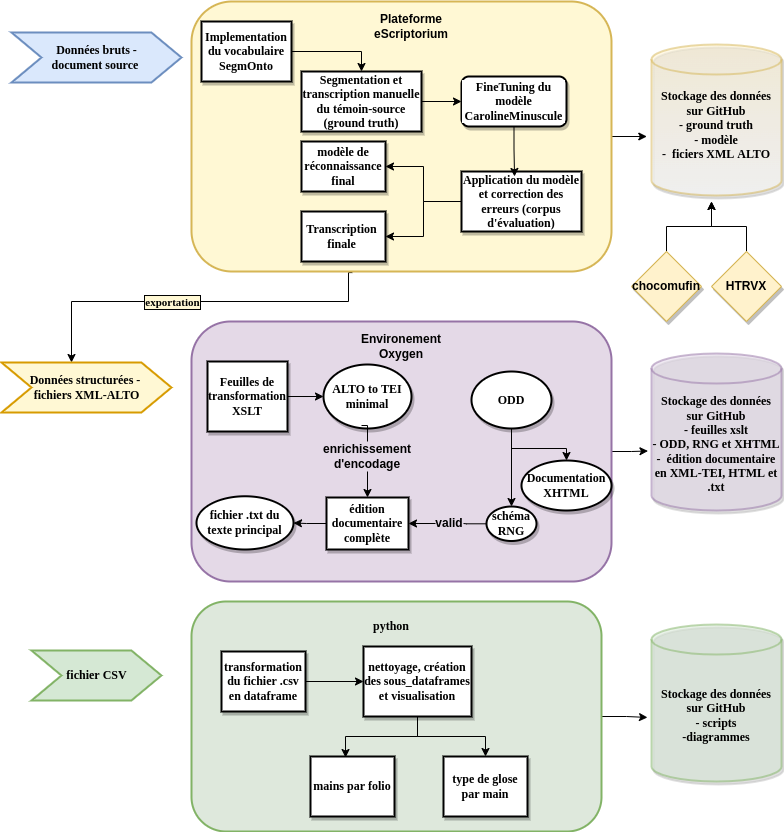
\includegraphics[width=18cm, height=17cm, width=17cm]{modelisation_pipeline.png}
    \caption{Modelisation du pipeline suivi. Trois niveaux de traitement successifs, de la transcription à la structuration et la visualisation des données.}
\end{figure}

Le pipeline suivant a été pensé en prenant en compte tous les aspects dont : les besoins, les objectifs, les outils, les enjeux techniques, les résultats attendus, le type d’analyse sur textes extraits, et les résultats voulues. Idéalement, l'objectif de ce projet est le développement d'un pipeline englobant qui prend en compte les spécificités de tous nos témoins.

\section{Aquisition des données : HTR}

Il existe de nombreux logiciels d'OCR (Reconnaissance Optique de Caractères) et d'HTR (Reconnaissance automatique de structure et d’écriture manuscrite) : Il s’agit de la conversion d’un texte imprimé, écrit ou inscrit, en un texte encodé par une machine par un logiciel de reconnaissance automatique de texte qui analyse une image numérisée pour en extraire le texte. Certains sont propriétaires et d'autres sont gratuits, et ils ont tous des spécificités qui les rendent plus adaptés à un projet plutôt qu'à un autre. En ce qui concerne le logiciel utilisé pour le projet sur Eutychès, nous avons utilisé kraken \footnote{ \url{https://kraken.re/master/index.html}}, via son interface \textit{eScriptorium}\footnote{\cite{kiessling2019escriptorium}}, un outil d’analyse de mise en page et d’HTR fondé sur de l’apprentissage profond (IA). Ce choix s'explique par deux raisons principales. Tout d'abord, il s'agit d'un logiciel libre avec une documentation étendue (que ça soit des tutoriels en ligne ou la documentation dans leur \href{https://gitlab.inria.fr/scripta/escriptorium}{dépôt GitLab}). Pour ce qui est de plus, le personnel de l'ENC et d'Inria a activement et extensivement travaillé sur plusieurs projets en utilisant \textit{kraken} et eScriptorium\textit{}, ce qui a facilité considérablement à resoudre des problèmes que nous avons rencontrés au fur et à mesure de notre recherche, qu'ils soient d'ordre technique ou méthodologique. 

\subsubsection{ Analyse de la mise en page complexe / Complex Layout Analysis}

La première étape vers l'acquisition de nos données, dans notre cas les différentes couches de texte contenues dans la copie numérique des folios de VLO41, est leur segmentation. La segmentation constitue le processus qui consiste à décomposer l'image entière en sous-parties pour les traiter ensuite. Dans el cas du VLO41, la segmentation de l'image est effectuée dans l'ordre suivant : segmentation au niveau de la zone et segmentation au niveau de la ligne. \textit{Kraken} propose déjà un modèle par défaut pour la segmentation des pages écrites de gauche à droite, entraîné sur un grand ensemble de données, qui traite assez bien les lignes principales de la page, à condition que la qualité de l'image soit bonne. Néanmoins, compte tenu des spécificités susmentionnées et de l'hétérogénéité considérable de la mise en page, la segmentation de la page avec le modèle integré n'était pas dans tous les cas capable de gérer la localisation inattendue de l'information, comme par exemple plusieurs lignes interlinéaires ou marginales écrites en petits caractères. Il n'était pas rare non plus pour le modèle de confondre le texte avec le paratexte, en mélanger les lignes principales avec les lignes interlinéaires ou marginales. Face à cette gestion incomplète et afin de conserver la mise en page et la hiérarchie inhérente aux différents niveaux, une approche manuelle et personnalisée a été adoptée pour la segmentation de chaque page. Cette étape de \textit{Complex Layout Analysis} consiste à détecter les zones d’intérêts : c’est-à dire les zones de textes, la pagination, les colonnes, les reclames etc. ; éventuellement, il s'agit de différencier les niveaux sémantiques distincts qui coexistent dans une image. 

Dans ce cadre, la stratégie suivante a été mise en place : chaque ligne principale a été notée comme telle du début à la fin, en constituant une unité sémantique. Par contre, il n'en a pas été de même pour l'espace interlinéaire. En effet, une ligne interlinéaire était séparée en autant de lignes que de gloses présentées en son sein. Et cela parce que la disposition spatiale au sein de l'espace interlinéaire ne correspond pas à une line où existe un flux continu de sens. Les gloses interlinéaires, en tant qu'extensions du texte principale, n'étaient pas conçues pour être lues l'une après l'autre de manière linéaire. Cette approche a été mise en oeuvre a priori comme un moyen de donner aux gloses un statut d'autonomie tenant compte également de l'extraction et exploitation des données. Alors dans notre système, une ligne dans l'espace interlinéaire vaut pour une glose, celle si s'afférant à un lemme. En revanche, comme c'est le cas avec les manuscrit d'usage, la situation n'est pas aussi simple qu'une modelisation simpliste en fait. Au moins pour les interlignes, dans de rares occasions (4 au total) les gloses s'étalent sur deux lignes au lieu d'une, rendant inopérante la règle 1ligne=1glose.Étant donné cette petite exception (4/~1050) à la règle générale, veillant à l'uniformité de nos données, nous avons fait le choix éditorial de transférer la moitié inférieure vers la moitié supérieure de la glose, en ajoutant le signe "/" pour signaler le saut de ligne existant dans le manuscrit. Par exemple, pour la glose \textit{multitudo ho/minum} sur \textit{uulgus} qui se trouve dans la ligne 21 du folio 11r, la barre verticale oblique indique le saut à la ligne. Cela constitue une des limites de notre segmentation, notamment en ce qui concerne la validité de la verité de terrain\footnote{ La verité de terrain consiste en\og{}des ensembles de données annotées et corrigées de manière à fournir au modèle des paires composées d'une part d'une image ou d'une portion d'image (entrée) et d'autre part de l’annotation attendue (sortie), qui peut être des coordonnées dans le cas de la segmentation ou un ensemble de caractères pour la transcription. Les performances des modèles dépendent certes de l'architecture neuronale mise en place, mais aussi de la qualité et de la quantité de vérité de terrain fournies lors de l'apprentissage.\fg{} Définition tirée de \cite{chague2021htr}}, par contre indispensable pour la manipulation des données. \\

\textsc{SegmOnto}


Dans la même veine, une opération complémentaire a été également adoptée, en faisant usage des vocabulaires controlés.
Un vocabulaire contrôlé est un lexique dont le but est de permettre l'organisation des connaissances pour optimiser la recherche d'informations. Le vocabulaire contrôlé est utilisé dans les schémas d'indexation par sujet, les thésaurus et les taxonomies et nécessite l'utilisation de termes prédéfinis qui ont été présélectionnés par le concepteur du vocabulaire.  Afin de repérer les différentes zones du document et le type de lignes présentes dans la page ainsi que de les caractériser d'un point de vue codicologique, nous avons décidé d'implémenter le vocabulaire contrôlé SegmOnto \footnote{\cite{gabay2021segmonto}}. SegmOnto est né du besoin pour une application informatique d'un vocabulaire commun limité, une ontologie basé sur les normes existantes, pour la description et l'analyse de la mise en page de documents, allant de la catégorisation du contenu à la reconnaissance de texte. SegmOnto aborde principalement le cas des manuscrits, ce qui favorise davantage son utilisation. Cette pratique répond aux bésoins de plus en plus pressants dans le domaine de l' HTR. En effet, avec l'apparition d'analyseurs de mise en page efficients et d'interfaces faciles à utiliser, le besoin de modèles efficaces de segmentation augmente, tout comme le besoin de grandes quantités de données, basée sur l'agrégation de documents hétérogènes. Pour cela, les chercheurs doivent a se mettre d'accord sur un vocabulaire commun limité,et partager des pratiques communes pour faciliter l'interopérabilité de leur vérité de terrain. En s'adhérant à ce cadre scientifique et en reconnaissant les avantages d'une méthode de description -dotée d'une empreinte numérique sur l'export en format ALTO- pour les documents hétérogènes à plusieurs niveaux, nous avons implementé SegmOnto pour VLO41.\\

En pratique, la caractérisation des zones et des lignes est très adaptée au cas du VLO41, étant donnée les doubles contraintes de la mise en page où l'ordre de lecture est perturbé, et les trois niveaux d'information que l'ajout des gloses impose. Prenons l'exemple d'application le plus manifeste : Considérant qu'eScriptorium fait une lecture horizontale les lignes en allant de gauche à droite, les colonnes, introduisant une lecture verticale, sont ignorées\footnote{Et pour citer Mr. Vidal-Gorène dans un récent entretien pour BULAC (cf. supra n.9) : \og{} Ainsi pourrais-je obtenir un CER* de 0\%, mais si les lignes ne sont pas lues dans le bon
ordre, est-ce pour autant utile ?\fg{} }. Par conséquent, tracer manuellement les différentes \og{} zones de lecture \fg{} avec SegmOnto est une condition indispensable. La page se divise ainsi dans les zones suivantes selon l'information qu'elle portent:

\begin{itemize}
    \item \textit{NumberingZone} pour la foliotation ;
    \item \textit{MainZone}, ou eventuellement \textit{MainZone}\#1,\#2 et ainsi de suite pour la zone qui comporte le texte principale ainsi que les gloses ;
    \item \textit{MarginTextZone} pour les gloses marginales ;
    \item \textit{MusicZone} pour les neumes ;
    \item \textit{GraphicZone} pour les dessins.
\end{itemize}

Il en va de même pour les deux types de lignes. Grâce à SegmOnto, les deux niveaux d'information, les lignes principales ( marquées en tant que \textit{DefaultLine}) et les interlignes (marquées en tant qu' \textit{InterlinearLines}) peuvent être distinguées et caractérisées, ne laissant aucune ambiguïté sur la nature de la ligne en question, tout en facilitant l'extraction et l'exploitation des données. En outre, afin d'assurer un contrôle qualité de notre export lors du stockage des information sur GitHub, le logiciel \textit{HTRVX}\footnote{\cite{Clerice_HTRVX_HTR_Validation_2021}}, développé  par Thibault Clérice et Ariane Pinche a été mise en place vérifie le schéma XML et l’utilisation de l’ontologie Segmonto pour la segmentation. \\


Des exemples de gestion du zonage et des lignes sont présentés dans la Figure 2.2  ci-dessous :

\begin{figure}[H]
    \begin{subfigure}{0.40\textwidth}
    \centering
    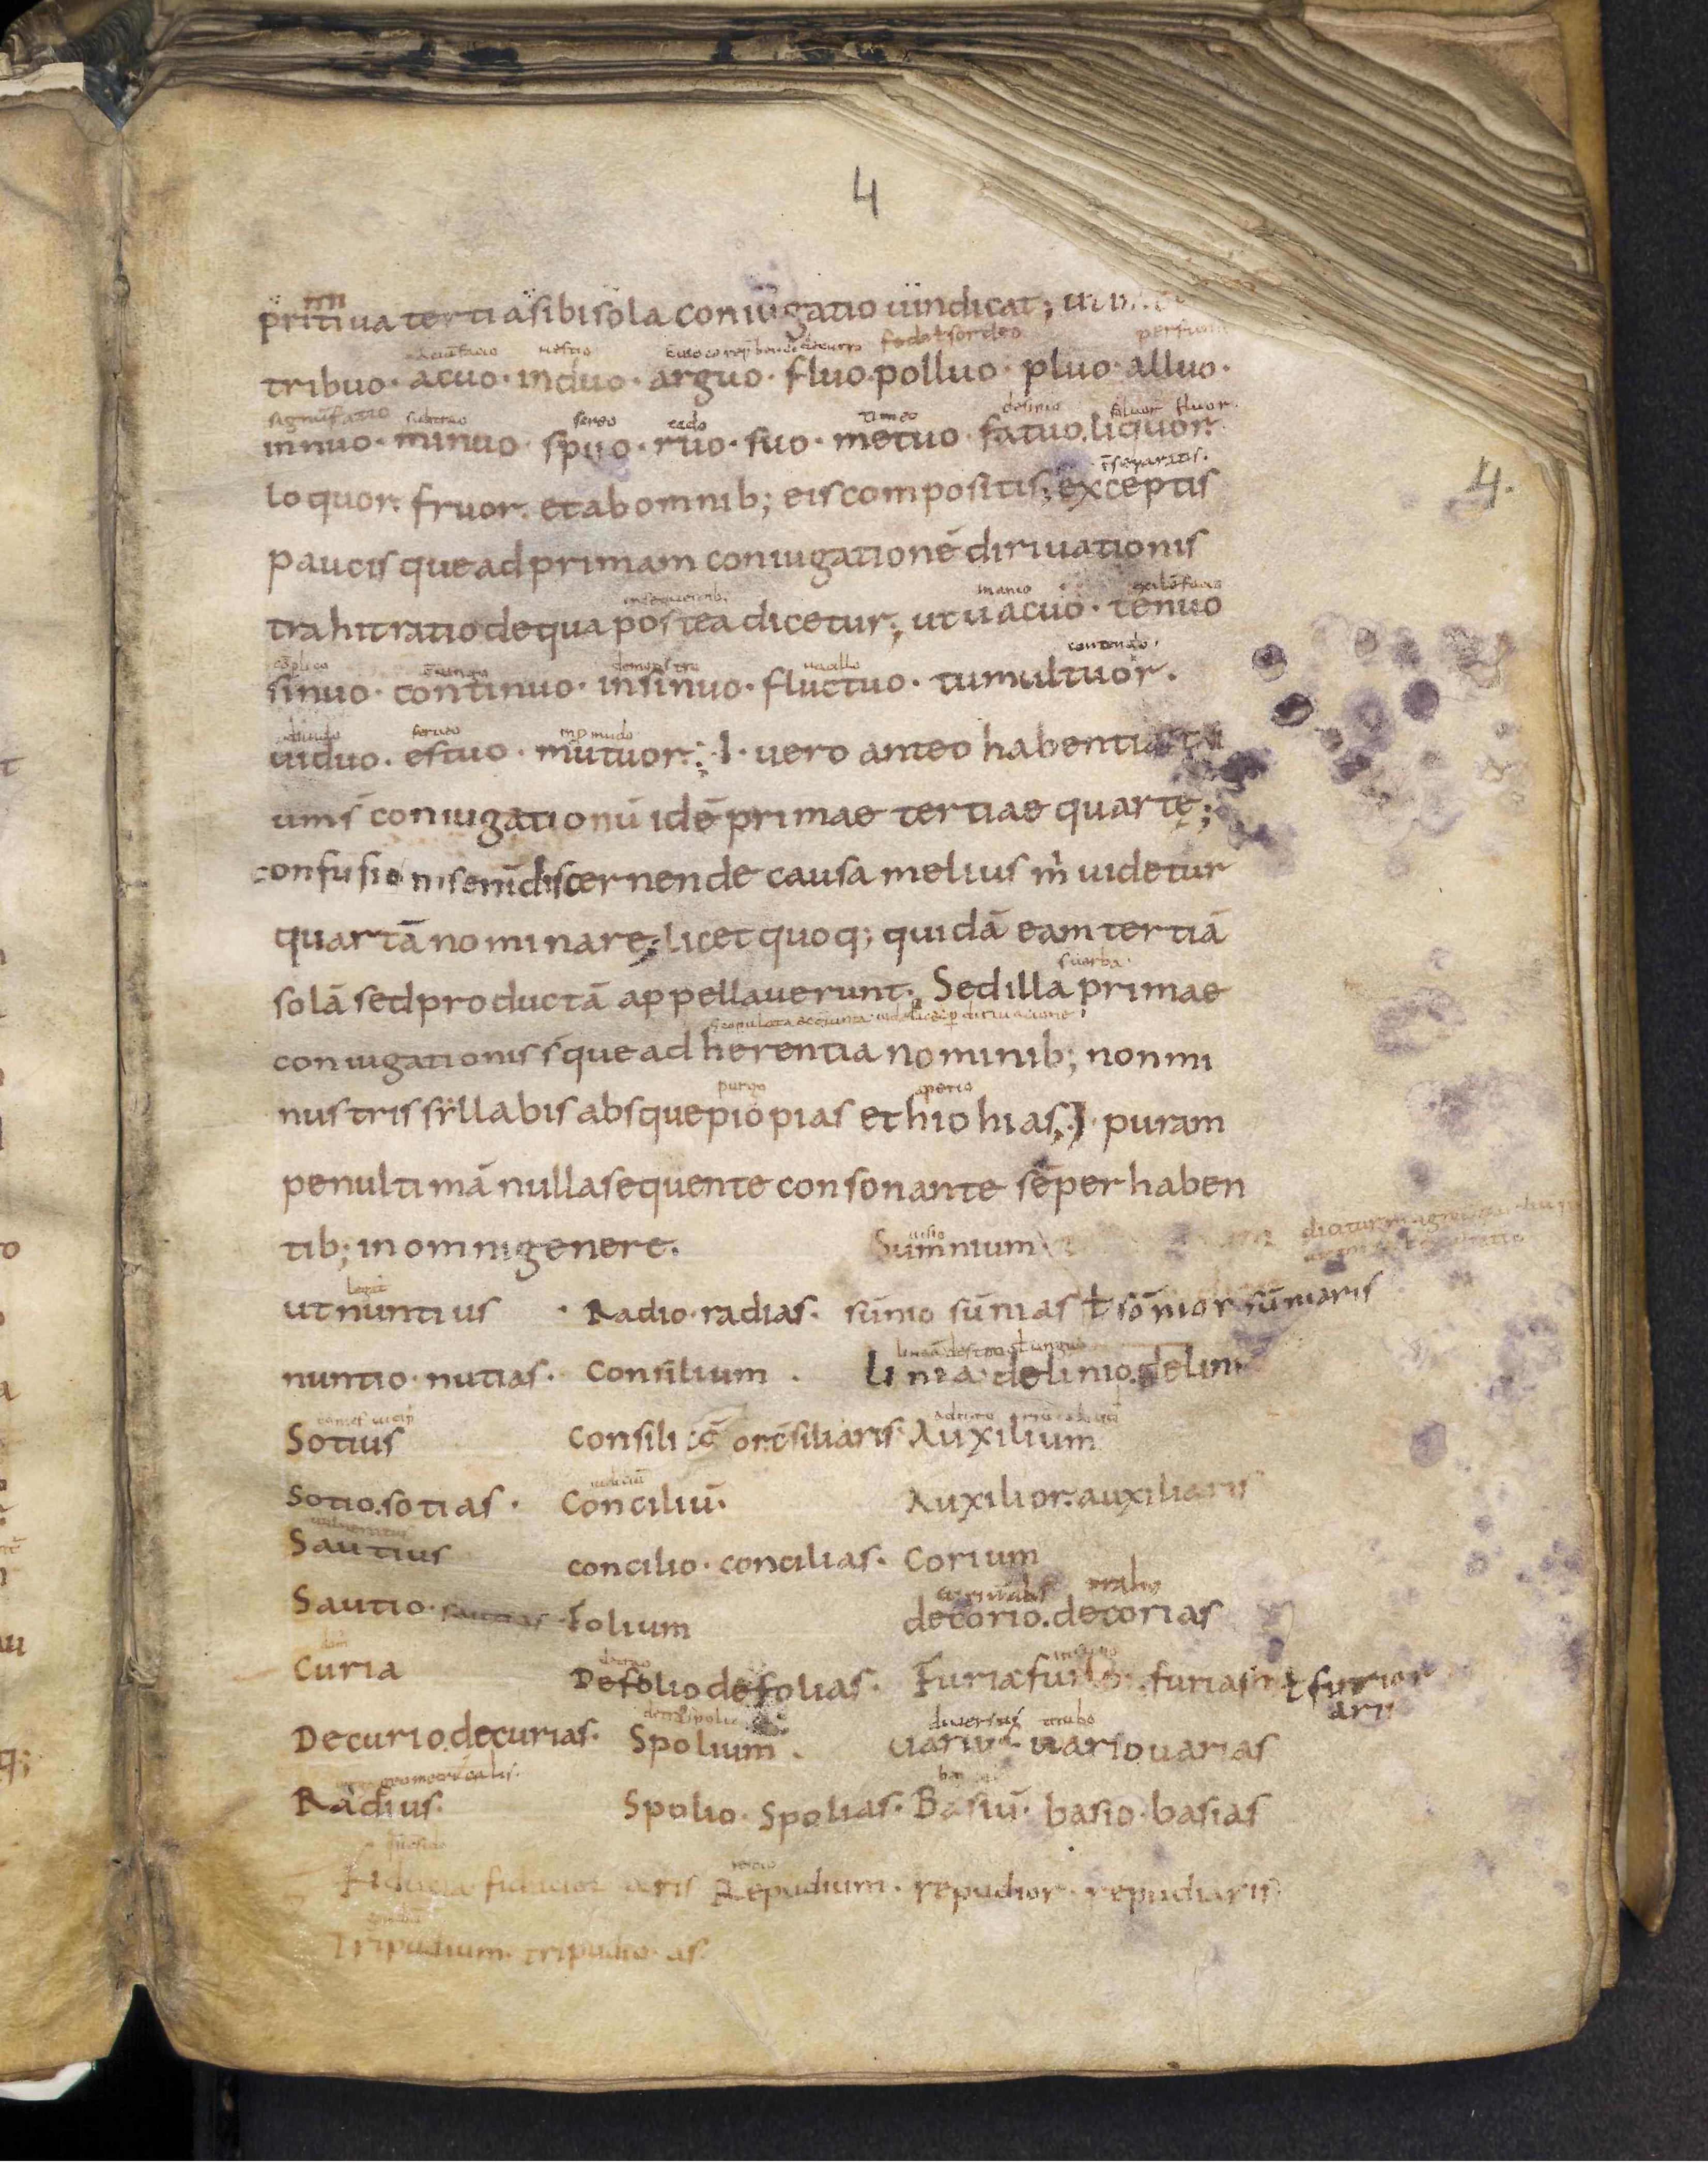
\includegraphics[width=7cm]{4r.png}
    \caption{folio 4r}
    \end{subfigure}
    \begin{subfigure}{0,40\linewidth}
    \centering
    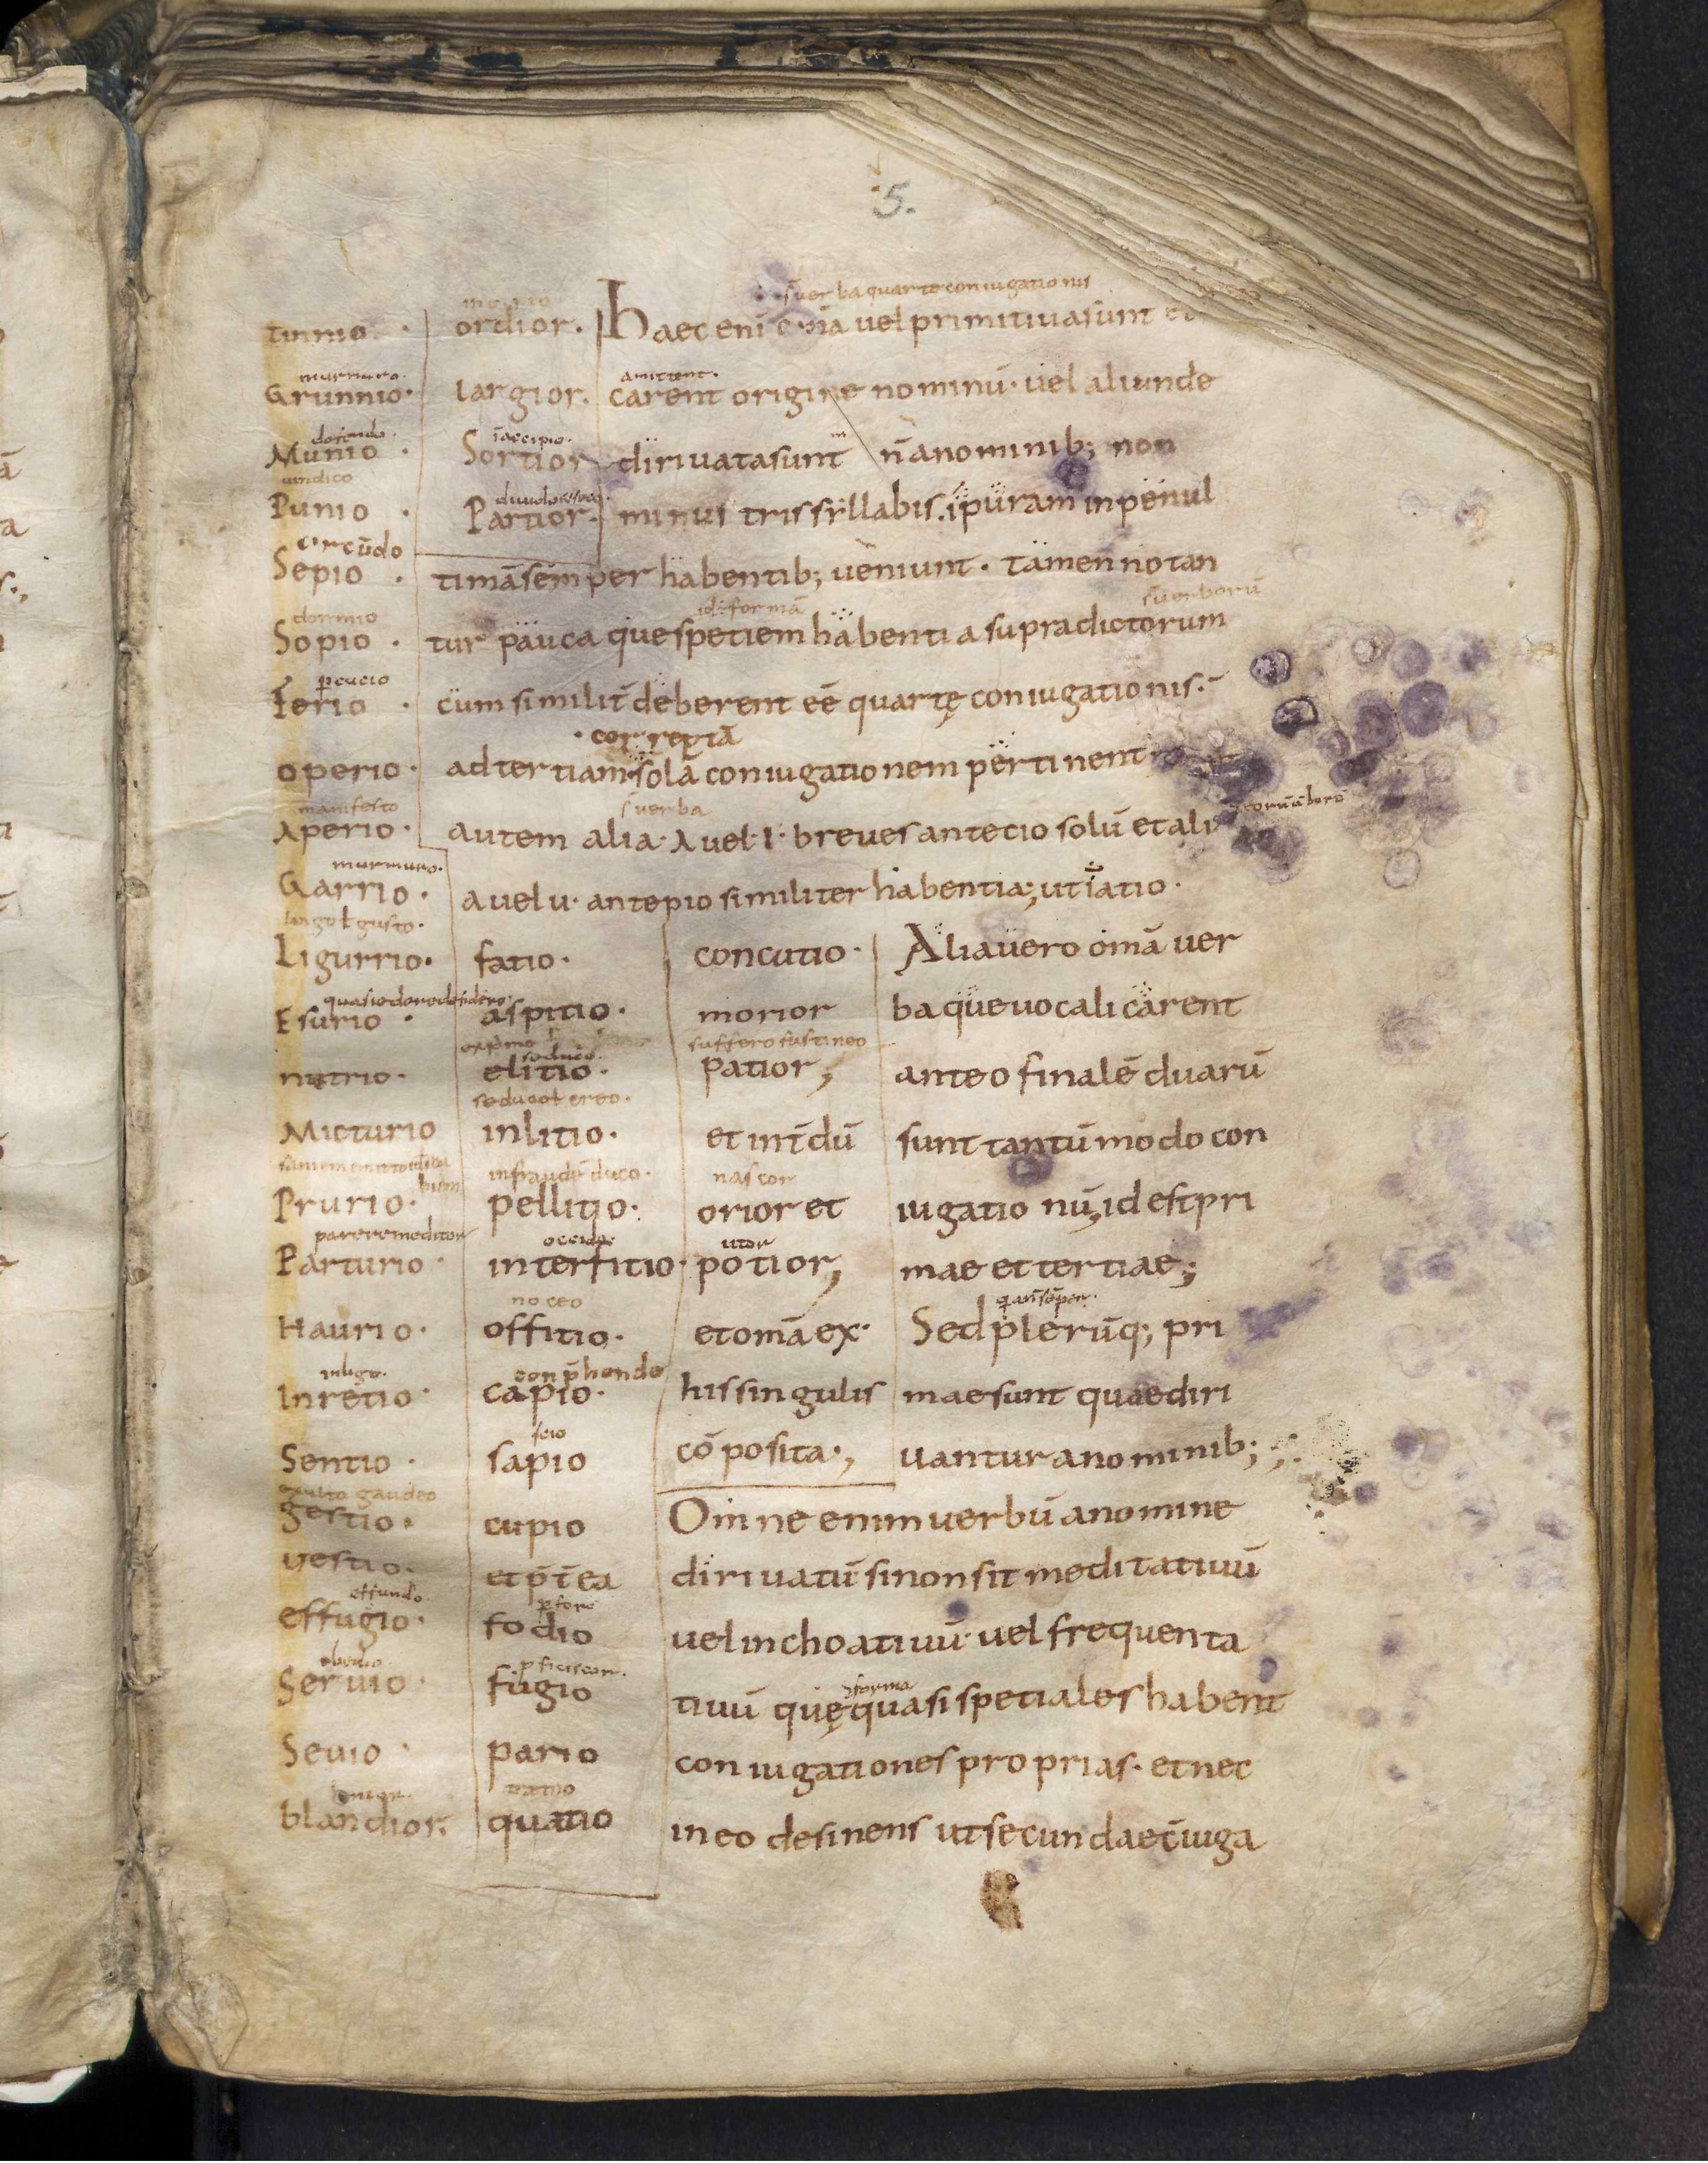
\includegraphics[width=7cm]{5r.png}
    \caption{folio 5r}
    \end{subfigure}
     \begin{subfigure}{0,40\linewidth}
    \centering
\includegraphics[width=7cm, height= 10cm]{3r_Lignes_Segmonto.png}
    \caption{ folio 3r }
    \end{subfigure}
    \caption{ (a) et (b) Disposition des zones SegmOnto afin de rétablir le sens de lecture. (c) DefaultLines en rose, InterlinearLines en orange. }
\end{figure} 


\subsubsection{Reconnaissance}

Jusqu'à très récemment, les anciennes écritures manuscrites telles que la minuscule caroline ont été considérées comme imperméables aux outils de transcription automatique comme kraken. Certes, il était toujours possible d'entraîner des modèles sur un ensemble de données, mais un modèle générique \og{} clé en main \fg{} capable d'atteindre une précision élevée générale pour plus qu'un manuscrit n'était pas facile à mettre en place \footnote{Sur la complexité que la minuscule caroline pose et les facteurs qui entrent en jeu lors du melange des modèles différents voir l'article : \cite{hawk2018modelling}}. Depuis 2019 et l'avancement des moteurs OCR qui gèrent les écritures manuscrites, cette difficulté a été partiellement resolue, en permettant une plus grande interoperabilité entre modèles HTR. \\


Un tel modèle \og{} clé en main \fg{} nous avait été fourni par Mr. Thibault Clérice \footnote{Pour la vérité de terrain de ce modèle voir. \url{https://github.com/rescribe/carolineminuscule-groundtruth}. Le protocole de transcription s'aligne à 100\% avec nos propres normes de transcription, qui visent une approche autant que possible graphématique.} qui, à l'époque, atteignait le taux de précision  de près de 92\%. Tout de même, une fois appliqué, celui-ci  nécessitait
uen grande campagne de post-correction pour notre manuscrit. En effet, en raison de l'estompage considérable de l'encre, le modèle n'était pas efficace pour l'ensemble des pages. Et bien sûr, cela ne concerne que le texte principal et en aucun cas les gloses de petite taille qui l'entourent. Il est important de noter que l’efficacité de la reconnaissance des caractères et des mots à proprement parler dépend directement du travail réalisé sur la segmentation de la page. En d’autres termes, même si le modèle de reconnaissance des caractères est performant, une segmentation incorrecte ou
incomplète empêchera tout résultat satisfaisant. Pour toutes ces raisons, la plus grande partie de la transcription a été faite manuellement, dans l'optique de \textit{fine-tuner} ou plutôt de personnaliser le modèle fourni pour qu'il réponde à nos bésoins \footnote{ \og{} Fine tuning ou spécialisation progressive : Il s’agit, dans le domaine de l’intelligence artificielle, d’adapter un modèle préexistant à un jeu de données spécifique à la tâche visée.\fg{} L'ensemble du vocabulaire specialisé HTR et une description minutieuse de la chaîne de traitement se trouve dans l'excellent rapport rédigé par Noëmie Lucas, dans le cadre d'une résidence de recherche à la BULAC en 2020-2021 soutenue et publié par le GIS, an libre accès en ligne \url{http://www.bulac.fr/node/2491}
}. 80\% du jeu de données, a été reservé pour le \textit{fine-tuning} et 20\% pour l'évaluation. La presence de, au total, huit mains distinctes dans le meme jeu de données offre une variété précieuse qui empeche une surapprentissage totale sur une des mains et l'impossibilité d'une reutilisation directe du modèle de réconnaissance. Par contre, dans la selection de la verité de terrain les pages fortement annotés, où les masques des lignes interlinéaires se superposent avec ceux des lignes principales à tel point  que la verité de terrain est \textit{contaminée},ont été écartées. Le modèle final, d'un taux de 98,4\% d'accuracy \footnote{disponible ici: \url{https://github.com/malamatenia/Eutyches/tree/main/data/models}}, a été employé pour la transcription des trois pages du glossaire BnF.lat.14087 (corpus de test) qui a necessité une post-correction minimale. \\


Afin de vérifier la qualité de notre lecture, au moins pour ce qui est du texte principal, nous avons comparé notre transcription avec celle de Keil\footnote{\cite{keil1857grammatici}}. Cela nous a permis de valider certaines de nos intuitions en cas de doute, de corriger certaines de nos erreurs et de mettre en évidence les endroit où le témoin s'écarte de l'édition de référence. Par contre, la lecture des presque 1050 gloses, n'a pas été toujours facile. La petite taille, le caractère informel de leur redaction et l'usure/moisissure du manuscrit n'ont pas facilité notre tâche. Dans le cas de doute, nous avons mobilisé plusieurs stratégies. En premier lieu, les autres témoins glosés\footnote{Notamment le BnF.lat.7498, le glossaire BnF lat. 14087 et le BL MS. Auct. F. 4. 32 avec qui VLO41 partage une bonne partie des gloses et dont l'écriture, très lisible ne laisse pas des doutes sur la lecture.} nous sont servi comme base comparative contre laquelle nous avons pu vérifier la lecture, notamment pour ce qui est des synonymes. Dans le cas où une étude coisée n'est pas possible, absence de correspondances entre témoins, des fouilles exhaustives dans la Database of Latin Dictionaries(DLD) et dans la Library of Latin Texts de Brepolis ont élucidé les propos des glosateurs \footnote{Je tiens à rémercier aussi Mme. Conduché pour la lecture de la glose \textit{reicio} sur \textit{repudium}, en bas du folio 4r., une lecture pas évidente à cause de l'usure du manuscrit}. Cette méthode nous a permis une lecture aussi fiable que possible des gloses,  avec bien sûr peu de \textit{loci} vraiment \textit{desperati}. \footnote{Tous les passages restitués sont méticuleusement signalés dans le fichier XML-TEI à l'aide de l'élémént <supplied> qui permet d'enregistrer aussi le taux de certitude d'une lecture proposée.} \\

En ce qui concerne les normes de transcription, le texte a été transcrit aussi fidèlement que possible, avec une intervention minimale de notre part\footnote{Une approche purement graphématique a servi, entre autres, à une verité de terrain propre pour le \textit{fine-tuning} du modèle de base.}. Les caractères diacritiques, les signes spéciaux\footnote{Sauf un signe, qui ressemble à un \textit{s} tironien et qui sert d'abréviation du \textit{scilicet} qui introduit des gloses ecplicatives, a été transcrit en tant que \textit{s}} et les abréviations et la ponctuation mediévales ont été conservés éléments précieux pour les collations eventuelles pour l'établissement du texte, nécessitant toujours une nouvelle édition \footnote{Aux chantiers par Mme. Condcuhé.}. Par contre, une intervention a été necessité pour la gestion des espaces entre mots dans les premières page qui presentent des caractéristiques d'une \textit{semi-continua}.\\

Finalement, comme il était le cas pour la segmentation, lors du stockage des données, le logiciel \textit{Chocomufin}\footnote{ qui vaut pout CHaracter Ocr COordination for MUFI iN texts\cite{Clerice_Choco-Mufin_a_tool_2021}} a été mis en place. Il s'agit d'un outil permettant de normaliser l'utilisation des caractères spéciaux issus de \textit{mufi}\footnote{The Medieval Unicode Font Initiative: \url{https://mufi.info/m.php?p=mufi}} et de vérifier la cohérence des fichiers XML. Il cible principalement le traitement des manières trop diverses de transcrire les données médiévales (allographiques et graphématiques) tout en conservant des informations telles que les abréviations. La validation \textit{chocomufin} confirme la compatibilité de notre verité de terrain avec le projet \textsc{Cremma}\footnote{\url{https://github.com/HTR-United/CREMMA-Medieval-LAT}} permettant une interoperabilité des données et leur réutilisation pour l'entrainement des modèles de réconnaissance automatique. \\

\textsc{Alto}

Une fois le texte segmenté, annoté et transcrit, il reste de décider le format qui se prête le mieux à l'exploitation des données structurées. Entre format .txt, PAGES et ALTO qui sont proposés par eScriptorium, le format ALTO est le plus adapté aux bésoins du projet. Il va sans dire que le format .txt brut n'est pas du tout adéquat,du fait qu'il ne respecte pas ni reflêt l'hierarchie interne de la mise en page et du contenu, sans parler du fait qu'il est illisible en raison de la confusion des lignes. En revanche, le format XML-ALTO (Analysed Layout and Text Object)\footnote{\url{https://www.loc.gov/standards/alto/}},qui est un standard XML permettant de rendre compte de la mise en page physique et de la structure logique d'un texte transcrit par reconnaissance optique de caractères (OCR) est, donc, essentiel. De plus, il est adapté à la conservation à long terme des données issues de la conversion OCR et permet une réutilisation et transformation des données en des formats différents, ce qui constitue précisément notre prochaine étape.\\

\section{Transformation des données}

\subsection{XSL}

Le format ultime que nous souhaitons atteindre c'est une édition documentaire en XML-TEI. Pour y arriver, il est impératif de transformer la sortie de notre transcription, à savoir les fichiers XML-ALTO en XML-TEI\footnote{\cite{janes2021towards}}. A ce but, et afin de mettre en valeur l'annotation SegmOnto, nous avons choisi d'utiliser des feuilles XSL\footnote{ Accessibles dans : \url{https://github.com/malamatenia/Eutyches/tree/main/XSL}}. A partir de la structure des fichiers ALTO et en appliquant des règles propres à une transformation vers un format XML-TEI valide, nous avons pu obtenir le squelette\footnote{\url{https://github.com/malamatenia/Eutyches/blob/main/XSL/out/VLO41_ALTO2TEI_minimal.xml}} d'un fichier TEI, avec toutes les informations codicologiques concernant la foliotation, les lignes principales, les interlignes, et les commentaires en marge annotées avec SegmOnto. La Figure 2.3 represente une modelisation de cette transformation ALTO vers TEI. \\

\begin{figure}[H]
    \centering
    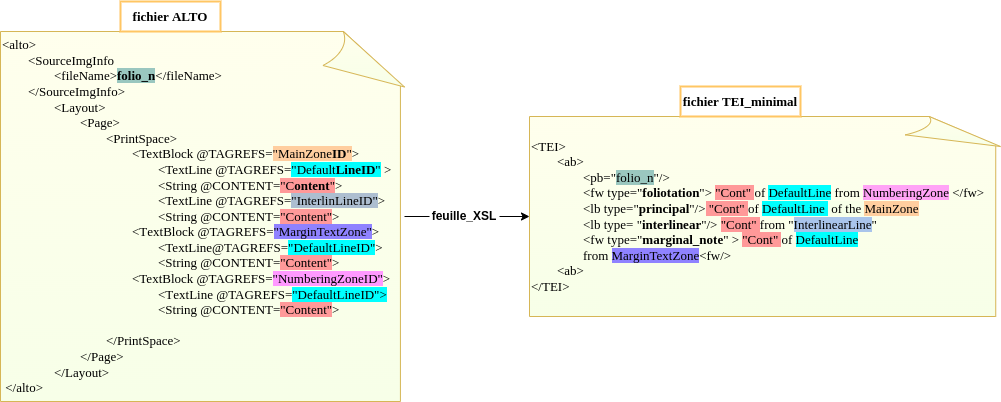
\includegraphics[width=15cm, height=8cm]{ALTO_to_TEI.drawio.png}
    \caption{ Transformation des fichiers ALTO à un fichier XML-TEI minimal avec integration de l'ontologie SegmOnto }
\end{figure}


L'interopérabilité et la réutilisation des données, avec une possibilité de transformation en plusieurs format différents, se trouve au coeur des débats des Humanités Numériques et cela pas sans raison. Ainsi, au lieu de tout encoder à la main, une grande partie est structurée de façon automatique, ce qui permet d'économiser du temps tout en assurant la cohérence des données. Il ne reste que complèter l'encodage manuellement, en fixant les éléments d'intêret. Étant donnée les problématiques énoncé dans la première partie du mémoire, nous n’avons pas envisagé notre encodage comme une simple pratique d’édition, mais plutôt comme une pratique de recherche qui permettra l'interrogation et exploitation des données de manière la plus efficace.

\subsection{XML-TEI}

En se penchant sur la notion de l'édition critique, étant donné la distance entre l’original (\textsc{vi}\ieme{} siècle) et les copies (du\textsc{viii}\ieme{} au \textsc{ix}\ieme{} siècle), ce projet n’envisage ni de remonter à l’original ni de retrouver l’intention de l’auteur et la variante parfaite\footnote{\cite{cerquiglini1990eloge}}.Effectivement, la méthod(ologi)e lachmannienne a véhiculé l’idéologie de la reconstruction de l’\textit{Urtext} archétypique perdu, alors que tout texte connaît des réalisations différentes au cours de son histoire. Cela vaut particulièrement pour les éditions des gloses et des manuscrits glosés, où on considère  que \blockquote{l’ensemble des interventions faites par les acteurs qui l’ont produit constitue la recension primaire de la collection, quel que soit le nombre de strates qui la compose. [...] Dans le cadre de l’analyse des gloses décrit en termes de relations entre collections et corpus, le système stemmatique de Lachmann ne s’applique pas : il serait vain de vouloir faire remonter une collection de gloses à un modèle identique antérieur, puisqu’il n’a probablement jamais existé\footnote{ La même constatation fait Emmanuelle Kuhry, editrice du \textit{De plantis} glosé \cite{kuhry2020medieval}}. La démarche stemmatique [...] n'a aucun sens dans un contexte de transmission fluide. Il n’y a pas de texte « original » à reconstruire, sinon une source \og{} ultime \fg{}, modifiée et parfois transformée, de proche en proche, au fil des réemplois.\footnote{\cite{cinato2015priscien},p.260}}. Des méthodes et des outils d'analyse des relations entre collections et corpus de gloses qui offrent une plus grande souplesse se mettent à la disposition des éditeurs comme la phylogénétique et l'analyse des réseaux\footnote{cf. l'édition de \cite{steinova2021glosses}}. Le présent projet vise  simplement à mettre le texte dans son contexte \footnote{Pour une discussion sur les questions numériques que cette recontextualisation implique voir. \cite{pierazzo2011putting}} et à explorer les informations textuelles, paratextuelles et métatextuelles offertes par les témoins. Décontextualiser soit le texte de son paratexte soit l'inverse serait, pour citer Vivien Law \blockquote{rather like the fossil hunter who ignores the strata in which his prize specimen is embedded \footnote{\cite{law1997grammar},p.22}}.\\

Sur les fondements théoriques des éditions critiques numériques, Peter Robinson \footnote{\cite{robinson2001critical}} nomme six aspects essentiels à tenir en compte:

\begin{enumerate}
  \item Une édition numérique critique est ancrée dans une analyse historique des matériaux ;
  \item Une édition numérique critique présente des hypothèses sur la création et l’évolution dans le temps ;
  \item Une édition numérique critique fournit un enregistrement et une classification dans le temps, dans de nombreuses dimensions et avec des détails appropriés ;
  \item une édition numérique critique peut présenter un texte édité, parmi tous les textes qu'elle propose ;
  \item une édition numérique critique offre aux lecteurs l’espace et les outils pour qu’ils puissent développer leurs propres hypothèses et modes de lecture ;
  \item une édition numérique critique doit offrir tout cela de manière à enrichir la lecture.
\end{enumerate}

Tous ces critères peuvent être satisfaits dans un environnement numérique, tout en se souciant des spécificités du document à encoder. En effet, l’absence de contrainte spatiale permet de représenter les données dans leur totalité et la souplesse des outils numériques rend ces données permet une interogation plus efficace. Quoi qu'il en soit, pour que l'ensemble de l'information présente dans un manuscrit glosé soit exploitable, sa typologie précieuse doit être réproduite via l'encodage. Ce dernier doit fournir les moyens d’analyser l’ensemble des manifestations selon les différents niveaux d’informations qu'une typologie en \og{} multiple facettes \fg{} impose. Les questions essentielles sont liées à la structure, la sélection et l'encodage des données constituant le corpus. Ce corpus de gloses ouvrira autant de possibilités d'exploitation que le contenu des métadonnées sera organisé pour tenir compte des spécificités inhérentes aux gloses. La qualité des résultats et les possibilités offertes par le corpus dépendront de la richesse et de la variété des informations encodées : elles constitueront à la fois autant de critères de sériation que d'outils d'analyse. Dans l'ère du numérique, il n'est plus question d'encoder le plus grand nombre d'informations, mais plutôt de faire du document \og{} une synthèse structurée des variétés observables\og{}. Le contenu fondamental des collections - lemmes et gloses - devra être encodé de manière à permettre l'application de technologies visant à faciliter l'exploitation et l'exploration scientifiques des données. 


\subsection{Choix de l'encodage}

Dans cette section on va esquisser des stratégies de modélisation de l'encodage qui conviennent d'avantage aux manuscrits grammaticaux glosés, et qui remplissent au mieux les exigences d’un matériel et une typologie complexes, voire constituent une condition \textit{sine qua non}. Déjà les avantages d'une approche numérique concernant les manuscrits glosés ont été évoqués par Franck Cinato\footnote{\cite{cinato2015priscien} et \cite{cinato2011perspectives}} et Paolo Monella \footnote{\cite{monella2019digital}},qui ont travaillé et continuent à le faire sur la modélisation et l'encodage de la tradition manuscrite de Priscien de Césarée, et dont le travail a servi de point d'appui à notre processus d'encodage proprement dit. S'aligner sur les principales pratiques du domaine est crucial pour l'interopérabilité et l'homogénéité des données qui s'aprêtent à un examen vis à vis, comme pour le grand réseau de corpus des \textit{Grammatici Latini} \footnote{ Sur ce sujet la vision et l'entreprise majeure de l'Index Grammaticus déjà pendant les années '90 : \cite{lomanto1990index} et les perspectives d'un corpus éléctronique des GL décrites par Prof. Alessandro Garcea dans \cite{garcea2010corpus}}.\\

L'encodage doit fournir les moyens d’analyser l’ensemble des manifestations selon les différents niveaux d’informations dégagés précédemment. Face à ces niveaux, Franck Cinato a adapté des concepts développées dans le cadre plus large de l’organisation des connaissances sur le cas des manuscrits glosés, en suivant le \textit{faceted classification system\footnote{Une classification à facettes utilise des catégories sémantiques, soit générales, soit spécifiques à un sujet, qui se combinent pour créer la base de classification complète. Des facettes subordonnées affinent davantage le sujet.}}. Ces facettes permettent une caractérisation complète de l'éntite qu'on appelle glose, et consiste en plusieures dimensions, entre autres son emplacement (interlinéaire ou marginale) sa forme (signe, morphème,syntagme, phrase), son sens (classification qualitative selon l'apport d'une glose) et l'acteur (la main)\footnote{Pour l'éventail complet voir. \cite{cinato2015priscien}, Annexe 3}. L’intérêt qu’une  typologie complexe pendant la sériation permettra de réaliser réside en la  \og{}finesse granulométrique\fg{} dans les opérations de tri appliquées à de grands ensembles de données. Un encodage qui inclut l'ensemble des informations pivot, comme il sera mis en évidence lors de la visualisation des données (cf. \textit{infra}), qui s'avère particulièrement utile pour observer les mouvements de la confection du manuscrit et les préoccupations des glossateurs-compilateurs.\\

Le guide complet de l'encodage du texte se trouve dans le fichier ODD, disponible en version PDF et XHTML dans notre \href{https://github.com/malamatenia/Eutyches/blob/main/ODD/out/VLO41_edition_oddbyexample.pdf}{dépôt GitHub}. Nous nous contenterons ici de justifier la gestion de l'information multi-facette dans le choix de l'encodage. \\ 

\textsc{Mise en page}\\

En considérant que la mise en page joue un rôle fonctionnel plutôt qu'accessoire dans la disposition du contenu intellectuel de l'oeuvre, il est impératif que l'encodage inclue ces spécificités. En effet, la description
\og{} codicologique \fg{} qui s’attache plus à l’aspect formel des gloses, constitue une première facette du système d'analyse. Deux aspects qui méritent notre attention sont 1) la disposition en colonnes qui rompe le sens de lecture de l'horizontale à la verticale et 2) le type des lignes selon leur environement et leur fonctionnalité.\\


En ce qui concèrne la typologie des lignes, l'encodage, produit de la transformation XSL se presente ainsi : Les \textit{DefaultLines} se sont transformées en 
\begin{minted}{xml} 
<lb type="principal"> 
\end{minted}
et les \textit{InterlinearLines} en :
\begin{minted}{xml} 
<lb type="interlinear">
\end{minted}

Une spécification au niveau des lignes permet de la selection et l'extraction, en notre gré, soit uniquement du texte principal (utile pour la collation du témoin), soit uniquement des interlignes.\\


\textsc{Lemmes}\\

Comme il est déjà mentionnée, tout mot ou groupe de mots d'un texte principal forme potentiellement un lemme. Les lemmes, dans un sens ontologique contituent des segments arbitraires du texte principal qui se comportent en tant entités possédant un degré d'autonomie rélatif à leur dépendance du texte. Pour en fournir des exemples spécifiques, un verbe isolé (par exemple \textit{amo}) peut se suffire à lui-même, indépendamment du contexte immédiat ou intellectuel de la phrase. Par contre, un pronom (par exemple \textit{a quibus}) dépend entièrement de son contexte pour faire sens. Selon la définition du lemme adopté tout segment dont le sens a été augmenté en n'importe quelle manière, contstitue un lemme et est unique. \\

Côté pratique, un lemme est encodé ainsi:

\begin{minted}{xml} 
<seg type="lemma" xml:id="f02r_l01.2">nouas quęstiones</seg> :
\end{minted}

\begin{itemize}
    \item un élément neutre \textbf{seg} qui évite tout sémantisme en soi ;
    \item un attribut \textbf{type} = "lemma" qui spécifie la valeur sémantique du segment ;
    \item un \textbf{xml:id} composé des coordonnées du segment : ici il s'agit du deuxième lemme de la première ligne du folio 2r.
\end{itemize}

\textsc{Gloses in-situ et Gloses marginales}\\

En général, les gloses interlinéaires peuvent être non verbales, c'est-à-dire des signes de construction, des marques prosodiques, des chiffres (romains et plus tard également arabes), des petites lettres et d'autres symboles, ainsi que verbales, expliquant divers aspects introductifs mais essentiels du texte. Dans le domaine de la prosodie, les gloses traitent généralement des questions d'accents, de mètre et de techniques poétiques. Les questions de grammaire, tant morphologiques que syntaxiques, sont illustrés par la complétion de prépositions omises, l'explication des cas, la clarification des sujets et des objets, surtout lorsqu'ils sont exprimés par des pronoms (assez souvent dans VLO41), et l'aide concernant l'ordre des mots et la subordination des clauses. En matière de vocabulaire, les glossateurs proposent normalement des synonymes (rarement des antonymes, parfois la négation des antonymes), donnent des équivalents latins pour les mots grecs ou des traductions vernaculaires pour les mots latins, et fournissent des noms qui aident et enrichissent la compréhension du lecteur. En raison de leur nature très localisée, ces types de gloses sont généralement placés entre les lignes et à proximité de leurs lemmes, mais en raison de limitations particulières, ils peuvent être déplacés, parfois même jusqu'aux marges (cf. le premier critère du guide d'attribution des mains \href{https://github.com/malamatenia/Eutyches/blob/main/hand_attribution_guide.pdf}{ici}). Dans de tels cas, le jugement critique du lecteur est requis afin de les relier à la place qui leur est destinée dans le texte. Du point de vue de l'éditeur, toutes ces informations sont importantes et donnent un aperçu des pratiques pédagogiques qui découlent de la pratique des gloses.\\

Une typologie formelle des gloses attestées dans les manuscrits grammaticaux a déjà été formulée par Rijcklof H.F. Hofman\footnote{Hofman, Rijcklof HF. The Sankt Gall Priscian commentary. Part 1. 2. Translation and commentary; Indices. Nodus-Publ., 1996.} à la fin des années '90, typologie augmentée et épurée par Franck Cinato pour son édition de Priscien glosé. Cette facette \og{} Sens \fg{} consiste en sept souscatégories principales, à savoir :

\begin{itemize}
    \item S1 Prosodique
    \item S2 Lexicale
    \item S3 Grammaticale (morphologique)
    \item S4 Syntaxique
    \item S5 Explicative (commentaire)
    \item S6 Ecdotiques
    \item S7 Notes socio-historiques
\end{itemize}
 qui acceptent toutes des augmentations de sorte qu'il existe un chiffre unique pour toute manifestation sémantique de glose \footnote{Pour la typologie complète on renvoie à l'Annexe 3 de \cite{cinato2015priscien}}. Par exemple la typologie de loin la plus fréquente dans le VLO41 est la \textit{S22}, la glose lexicale qui procure un simple synonyme ou la \textit{S23} qui attribue une définition, ou bien la \textit{S54} qui propose une étymologie.
 
En même temps, bien qu’il faille prendre toutes les précautions nécessaires pour analyser ces données, il apparaît essentiel, pour l’établissement de la diachronie au sein des collections, de signaler les changements de scripteurs\footnote{Un petit guide des critères d'attribution des mains avec description détaillée et un échantillon se trouve dans le document \textit{hand\_attribution\_guide} de notre \href{https://github.com/malamatenia/Eutyches/blob/main/hand_attribution_guide.pdf}{dépôt GitHub}.}. Il convient d’abord de distinguer mains de copistes et de glossateurs. Par convention, on attribuera un chiffre aux copistes (mains 1, 2, 3, etc.) et une lettre aux annotateurs (mains A, B, C, etc.). En fonction du type de collection, les éléments du groupe lexical (lemme et glose) n’émaneront pas des mêmes personnages. \\

En pratique cette modelisation théorique donne l'encodage suivant : 

\begin{minted}{xml}

<lb type="principal"/> [...]gur auguro as, in as ut <seg type="lemma" xml:id="f11v_l22">nugas</seg> indeclinabile ut [...] 

<lb type="interlinear"/> 

    <gloss type="S22" xml:id="f11v_l22_a" target="#f11v_l22" resp="#B">
    uanꝰ  </gloss> 
    <gloss rend="italic" type="S23" xml:id="f11v_l22_b" target="#f11v_l22" resp="#A">
    recedens a lege</gloss> 
    <gloss type="S23" xml:id="f11v_l22_c" target="#f11v_l22" resp="#D">
    ł inutilis</gloss> 
    
\end{minted}


L'élément déjà défini\footnote{ Selon les Guidelines de la TEI : <gloss> (gloss) identifies a phrase or word used to provide a gloss or definition for some other word or phrase.} par la TEI \textit{gloss} est utilisé pour encadrer les gloses, suivi par l'attribut \@type qui sert à préciser la typologie mis en avant par Cinato. Pour ce qui est de plus, les gloses possèdent leur propre \textbf{xml:id} qui consiste en celui du lemme correspondant avec l'extension \textit{\_a} ou \textit{\_b} ou même \textit{\_c} selon l'ordre d'apparition au cas de plusieurs gloses afferant à un et le même lemme. Finalement, la main responsable est désigné par l'attribut \@resp. \\


Pour le contenu des gloses qui se trouvent en marge, annotées en tant que MarginalTextZone avec SegmOnto, et qui s'étalent souvent en plusieures lignes, sont encodés ainsi :

\begin{minted}{xml} 
<fw type="marginal_note" xml:id="f07r_l24.1_b" corresp="#f07r_l24.1" resp="#A">
       <lb type="principal"/> .s. nubo nubilis
       <lb type="principal"/> nubilis dr̃ apta ad
       <lb type="principal"/> muliem duxi 
</fw>
\end{minted}

L'élément <fw> (forme work), qui contient un titre courant (par exemple, un en-tête, un pied de page), un mot d'accroche ou un élément similaire apparaissant sur la page actuelle, sert comme element qui encadre la note marginale. De nouveau, suivant l'exemple des gloses interlinéaires, des \textbf{xml:id} y sont attribués et la main responsable est indiquée.\\



\textsc{Gestion des colonnes}\\

Un encodage propre aux colonnes, élément si important pour la transmission du texte, est adopté afin de sauvgarder l'ordre des lignes, ainsi que les couples lemmes-gloses présents en leur sein. L'exemple suivant est un extrait d'encodage de deux colonnes successives  du folio 4r (il en existe au total 3), dont certaines lignes principales sont glosées. De nouveau on se sert de l'élément <fw>, cette fois de \@type "colonnes" pour encadrer les groupes de colonnes. Au sein de cette structure, des elements vides <cb> numerotés, indiquent l'ordre d'apparition dans la page. 

\begin{minted}{xml} 
<fw type="colonnes" n="f04r">
        <cb n="1"/>
                              
            <lb n="01" type="principal"/> ut 
            <seg type="lemma" xml:id="f04r_c1_l01" >nuntius</seg>
                              
            <lb type="interlinear"/>
            <gloss   type="S22" xml:id="f04r_c1_l01_a" target="#f04r_c1_l01" resp="#B"> legatꝰ </gloss> 
                              
            <lb n="02" type="principal"/> nuntio. nutias. 
               
            <lb n="03" type="principal"/> 
            <seg type="lemma" xml:id="f04r_c1_l03">Sotius</seg>
                              
            <lb type="interlinear"/>
            <gloss type="S22" xml:id="f04r_c1_l03_a" target="#f04r_c1_l03" resp="#B">comes uicinꝰ </gloss>
                              
            <lb n="04" type="principal"/> Sotio. sotias 
                              
            <lb n="05" type="principal"/>
            <seg type="lemma" xml:id="f04r_c1_l05">Sautius</seg>
                              
            <lb type="interlinear"/>
             <gloss   type="S22" xml:id="f04r_c1_l05_a" target="#f04r_c1_l05" resp="#Α"> uulneratus </gloss>
                              
              [...]
              
        <cb n="2"/>
        
            <lb n="01" type="principal"/> Radio. radias.
                                    
            <lb n="02" type="principal"/> consilium 
                                    
            <lb n="03"  type="principal"/> consilior c̃siliaris
                                    
            <lb n="04" type="principal"/>
            <seg type="lemma" xml:id="f04r_c2_l04">conciliũ </seg>
                              
            <lb type="interlinear"/>
            
            <gloss type="S22" xml:id="f04r_c2_l04_a" target="#f04r_c2_l04" resp="#B">iudiciũ </gloss> 
            
             [...]
            
</fw>

\end{minted}

\textsc{Citations et \textit{Graeca}}\\

Au couple indissociable lemme-glosse et à la mise en page s'ajoutent deux aspects clés du \textit{De uerbo} et de sa tradition textuelle : les \textit{graeca} et les citations. Ces deux éléments,comme il a été déjà evoqué, ont une signification philologique et culturelle particulière pour l'histoire des textes linguistiques. 

Comme mentionné ci-dessus, le de uerbo a été composé à Constantinople, c'est-à-dire dans un environnement de langue grecque destiné à un disciple hellénophone, ce qui explique pourquoi Eutyches, cependant pas aussi souvent que son maître Priscien , compare les conjugaisons des verbes latins et grecs, et semble parfois traduire en grec afin d'expliquer le latin, principalement dans le deuxième livre. Si la présence des équivalents grecs répondait aux besoins du bilinguisme grec-latin de la Constantinople du VIe siècle, elle a ensuite posé un énorme problème aux scribes de l'Europe latine médiévale, qui ont progressivement perdu la connaissance du grec. Effectivement, si ils ne sont pas omis tout court, les \textit{Graeca} portent des erreurs significatives, precieuses pour la \textit{recensio}. Dans l'exemple suivantm tiré du folio 23v, Eutychès ressent le besoin de se référer au terme grec pour "fond", à savoir $\Pi \Upsilon \Theta \ M\ H\ N$, que le copiste a retranscrit avec l'orthographe phonétique, précieux indice pour la prononciation des termes grecs. \\ 

\begin{minted}{xml}
[...]a nomine qđ est fundus id est <foreign xml:lang="grc"> ΒΥΘΕΜΕΝ.</foreign>
\end{minted}


D'autre part les citations, tirées d'œuvres littéraires, sont également précieuses pour la \textit{recensio}. Ces dernières offrent une piste stable contre laquelle la \og{} Latinité \fg{} du copiste ou de l'exemplar peut être mise en examen.Une petite parenthèse concernant les citations des auteurs classiques et leur importance pour la transmission des savoirs pendant le Haut Moyen Âge : il suffit de mentionner que de toute la littérature profane, les manuscrits contenant les \textit{Artes} de l'Antiquité tardive sont les seuls qui soient parvenus à les conserver, de siècle en siècle. Même si on avait cessé de recopier Cicerón, Virgile, Horace, en continuant à recopier Donat, Charisius, Phocas, Priscien et les autres grammairiens de l'Antiquité tardive, que l'on a pu un jour reprendre goût à, lire et à recopier Virgile, Cicerón, Horace. Cette circonstance seule suffirait à établir que les manuscrits grammaticaux ne sont guère des recueils comme les autres\footnote{\cite{holtz1978typologie}, p.252}.Luca Martorelli, a dressé, en enrichissant les réferences de Lindemann \footnote{\cite{lindemann1833corpus}} une liste détaillée des 141 citations qui figurent chez Eutychès accompagnée des notes critiques sur les endroits où Eutychès d'écarte de l'original \footnote{\cite{martorelli2017citazioni}}.  C'est à l'aide de cette liste que nous avons pu localiser avec précision les nombreuses citations et leur associer un lien vers l'édition critique la plus récente, à condition que ça soit en ligne\footnote{notamment vers le {\href{http://www.perseus.tufts.edu/hopper/}{Perseus Digital Library}},ou bien sur {\href{https://archive.org/}{archive.org}}.}. Exemple d'encodage : \\

\begin{minted}{xml}
    <lb type="principal" break="no"/> VIII 
        <quote type="poetry"> has forte inuisitis aras
            <ref target="http://www.perseus.tufts.edu/hopper/text?doc=
            Perseus\%3Atext\%3A2008.01.0498\%3Abook\%3D1" resp="#LM"> 
            Stat. Theb. 1, 668</ref>
        </quote>
\end{minted}


Dans un environnement <quote>, on indique le genre auquel appartient la citation, prose ou poésie, ainsi que le responsable (@resp\footnote{Dans la plupart des cas, il s'agit de Luca Martorelli, sauf lorsque j'ai dû faire référence à une édition différente, disponible en ligne (et changer par la suite les coordonnées de référence). Dans ce cas la @resp est moi.}) des coordonnées de la référence (à l'intérieur d'un <ref>) et le lien (à l'aide de @target) vers le passage original.

Une granularité fine, adaptée à nos données, permet  l'exploitation du texte à deux volets. En premier lieu, preserver l'information de la mise en page, et en deuxième lieu, mieux interroger le texte en extrayant les balises d'intéret pour une comparaison interne ou entre témoins.

\subsection{Questions de normalisation/lemmatisation}

Bien que la TEI offre la possibilité de normaliser le texte tout en conservant les leçons originales, nous avons décidé de ne pas procéder à une normalisation. Ceci est dû à la nature particulaire du contenu grammatical et à la façon dont nous voulons traiter leurs propos. Et s'il est important d'utiliser les outils offerts par le numérique, tous les outils ne sont pas forcement adaptés à tout type de données.On est pas les premiers à être confronté à cette question. Déjà, dès les années '90, en exposant la méthodologie pour la confection de l' \textit{Index Grammaticus}\footnote{\cite{lomanto1990concordance}}, Valeria Lomanto et Nino Marinone se démandent quelle est la meillieure pratique à adopter pour étudier les co-occurences des termes dans le corpus des \textit{GL}. En considérant l'option de créer un \textit{Lexicon} (un thesaurus constitué des entrées d'un dictionnaire), ils rémarquent que : \blockquote{[...] it is not very \textit{suitable} for grammarians in that it involves \textit{lemmatization} and, as it provides \textit{no context}, it cannot reveal one of the salient characteristics of the\textit{artes}, namely its use of a sort of formulaic language present with \textit{slight variations} in every work. [...] The decision not to lemmatize derives both from the particular nature of the texts and from the future users of the concordance. In the \textit{artes} a high percentage of forms is represented by \textit{isolated graphemes} or by isolated morphemes or, in the chapters on metre, by units which are not linguistic but rhythmic (e.g. armaui rumqueca etc.). Moreover, lemmatization, while it requires a reliable critical text, necessarily
directs, if it does not condition, the interpretation.}

Une intervention éditoriale qui implique une corréction en masse des \og{} erreurs \fg{} que les copistes commettent, comme c'est le cas de la dmarche de Keil, va à l'encontre d'une étude scrupuleuse des variantes grammaticales utilisées par les copistes, qui donne des amples informations sur leur propre niveau de latinité. Pour reprendre les mots de Vivien Law\footnote{\cite{law1982insular},p.107}: 

\blockquote{It is of the utmost importance for future research that editors be scrupulous in their treatment of the texts before them. All departures from the text offered by the manuscripts should be signalled. Emendations, particularly in passages borrowed from Classical grammarians, should be undertaken sparsingly and indicated as such in the text. Editorial policy, with regard to orthography should be stated at the outset : the reader should be aware of how far the text before him differs from what a medieval student might have read. There is no justification when editing a medieval grammatical text for wholesale ‘normalisation’ to Classical conventions ; such a practice will cause havoc in alphabetical lists and reflect a miseleading image of the author’s latinity.} 

Une normalisation consiste à réduire les majuscules des noms communs, à uniformiser les orthographes multiples qui apparaissent pour un même terme sémantique, les dates et les chiffres et à développer les abréviations, pour procéder à une lemmatisation. La lemmatisation associe à ces graphies normalisées un lemme correspondant à l'entrée d'un dictionnaire et une catégorie grammaticale. Par conséquent, elle met au premier plan le niveau sémantique, puisque sa fonction principale consiste à définir les différents sens de chaque terme, à établir des relations de sens et à tracer la frontière poreuse entre polysémie et homonymie. Ce serait donc l'aboutissement d'une tradition philologique et exégétique si solidement ancrée, à l'issue d'une édition, qu'elle permet au savant d'affronter les problèmes de sens les plus délicats.\\

Pour ces raisons, nous avons opté pour une édition documentaire qui reflète au mieux l'état de la langue présenté par le manuscrit. Les éditions dites diplomatiques des grammaires pourraient constituer une ressource particulièrement précieuse pour les historiens de l'éducation et de la linguistique, car les enseignants et les penseurs médiévaux ne disposaient pas d'éditions critiques idéalisées dans leurs bibliothèques. Ils devaient se contenter des copies réelles à leur disposition, avec toutes les erreurs, les malentendus et les omissions qu'elles transmettaient. \\

\begin{figure}[H]
    \centering
    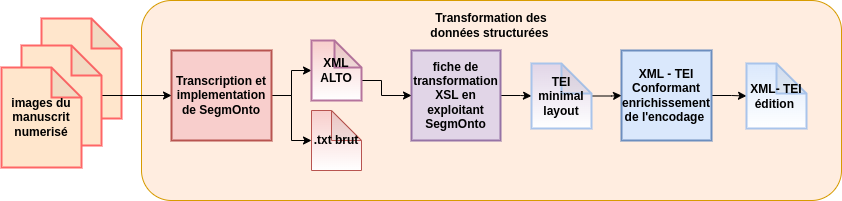
\includegraphics[width=18cm, height=4cm]{horizontal_pipeline_texte.png}
    \caption{ Rappel du pipeline  : Modelisation des opérations de transformation des données brutes en données structurées jusqu'à l'encodage complet (axe horizontale)}
\end{figure}


Après avoir effectué l'édition documentaire de notre témoin, il convient de se lancer dans la troisième étape, à savoir l'analyse exploratoire de nos données à multiples facettes. Un petit \textit{caveat} avant de continuer : Une utilisation plus propice de notre texte encodé en XML-TEI serait l'extraction des balises qui nous interessent dans un tableau .csv, pour la visualisation des données issues de l'encodage. Pour la première année du Master, nous nous sommes limités à manipuler un fichier .csv externe, compilé indépendamment du fichier XML-TEI et qui nous a servi de point de repère pour son encodage. Pour l'année prochaine, il contribuerait largement à l'homogénéité des données d'exporter les balises d'intérêt pour l'étape de la visualisation.


\section{Visualisation des données}


L’approche typologique des gloses, au-delà d’un simple classement, permet de mettre en évidence les préoccupations des glossateurs, ainsi que la spécificité de leurs enseignements \footnote{Toujours suivant : \cite{cinato2011perspectives}}. Il s’agit des informations \og{} externes \fg{}, liées à leur transmission, une sorte de métadonées, aspects d'aillieurs proprement paléographiques, qui se révèlent d’une importance primordiale dans le cadre de l’étude des gloses. La distinction des écritures détermine des éléments essentiels à l’analyse. Les premiers qui viennent à l’esprit ont trait à la distinction des mains qui ont laissé des couches superposées des gloses : un même manuscrit a souvent été étudié en différents lieux et à différentes époques. Il faut donc – pour rendre compte de la perspective diachronique au sein de la collection – établir une chronologie relative des mains qui ont participé à la formation du peri-texte. Cette étape n’est possible que dans le cas des sources de type $\Gamma$, comme le VLO.41. \\

Une facette spécifique \og{} Acteur \fg{} est prévue \textit{a priori} par Franck Cinato pour les mains différentes, en fonction du rôle de chaque glosateur, d'une echelle allant du 1 à 3 où:

\begin{itemize}
    \item A1 : Glossateur-copiste
    \item A2 : Glossateur-compilateur
    \item A3 : Glossateur-exégète
\end{itemize}

Faute d'experience de notre part et en se fondant sur un échantillon encore limité de données, nous avons decidé de de pas procéder à une \textit{a priori} attribution de rôles. En revanche, à l'aide des outils numériques, nous avons decidé de tenter une \og{} analyse exploratoire \fg{} sur les statistiques fournies par l'attribution des mains, aux fins de déterminer quelques charactéristiques propres à chaque glosateur. En effet, les outils numériques sont particulièrement adaptés pour la manipulation à large échelle et pour la visualisation des données à multiples facettes (comme le réseaux des gloses au sein du VLO41).

Ainsi grâce aux scripts python \footnote{Disponibles dans les notebooks de notre dépôt \url{https://github.com/malamatenia/Eutyches/tree/main/python-tools}} et la librairie \textit{matplotlib}, en choisissant des graphiques adaptés à nos données multi-variables, on a tâche à faire des observations générales sur les mouvements successifs d'annotation du manuscrit et sur les préoccupations différentes des glossateurs-compilateurs.\\

\subsection{Mouvements d'annotation}

Pour la première visualisation, nous nous sommes intéressés aux variables suivantes : la quantité de gloses écrites par et par folio, ce qui donne deux graphiques complémentaires (Figure 2.5 a et b).

\begin{figure}[H]
    \begin{subfigure}{0.50\textwidth}
    \centering
    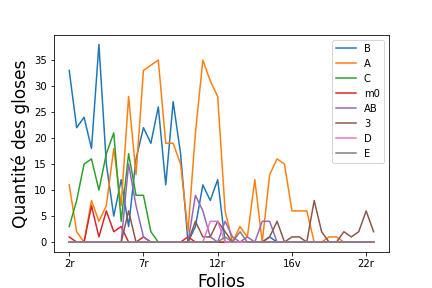
\includegraphics[width=9cm]{line_plot_hands_folios.png}
    \caption{line plot}
    \end{subfigure}
    \begin{subfigure}{0,50\linewidth}
    \centering
    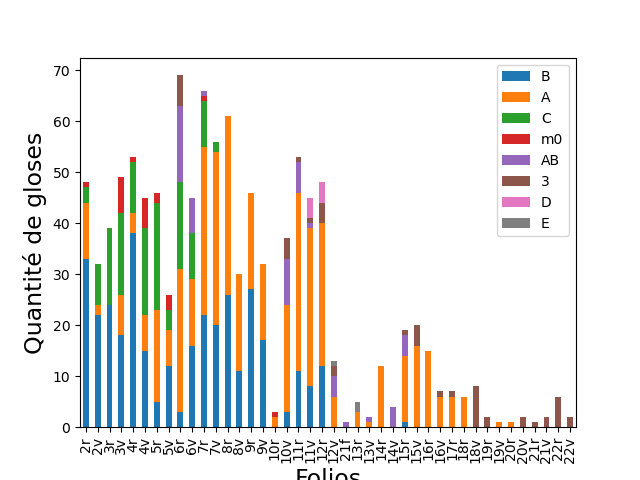
\includegraphics[width=9cm]{stacked_barplot_hands_folios.png}
    \caption{Stacked bar}
    \end{subfigure}
    \caption{Dans le premier graphique, une ligne correspond à une main en traçant sa contribution per folio. Le deuxième prend les mêmes variables et en donne la densité de la contribution de chaque main.}
\end{figure} 

\begin{figure}[H]
    \centering
    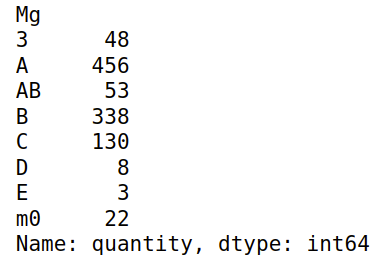
\includegraphics[width=6cm, height=4cm]{quantite_mains.png}
    \caption{Somme des gloses écrites par chaque main. "Mg" vaut pour Main de glosateur.}
\end{figure}


Le premier graphique permet de suivre le mouvement de chaque main par folios, l'intensité de leur activité au fur et à mesure.La seconde, complémentaire de la première, permet d'examiner plus en profondeur le pourcentage de contribution des mandants par folio, et l'émergence de tendances. Des observation d'ordre génerale peuvent être faites :

\begin{itemize}
    \item La quantité des gloses se diminue au fur et à mésure de la progression des folios, en confirmant la tendence générale qui atteste la concentration des gloses au début des manuscrits ;
    \item Le rôle marginal des 4 dernières mains est vraiment accentué par la visualisation. La main B est la main dominante pour les 5 premiers folios\footnote{Nous précisons ici que nous avons nommé les mains selon l'ordre d'apparition dans le manuscrit et non selon l'importance ou la quantité de gloses.},puis elle coexiste avec la main A jusqu'au folio 10v et la main A devient la main dominante jusqu'à la fin ;
    \item Trois mains apparaissent comme les principaux glossateurs du VLO41, à savoir A, B, et C. Alors que les deux premières ont une répartition plus équilibrée sur l'ensemble de la surface glosée, A prenant le relais après B, la troisième, C, se concentre uniquement dans les 14 premiers folios.
    \item On constanstate une absence générale de gloses dans le folio 10r.
\end{itemize}

Les observations quantitatives nous servent uniquement d'outil d'analyse et ne doivent pas être considérés comme une source suffisante d'interprétation. Néanmoins combinées avec les observations qualitatives, elles peuvent être nuancées et ainsi contribuent à des intepretations intéressantes, notamment quand il s'agit des corpus hétérogènes et multivariables. \\

Les deux dernières constatations méritent une élaboration plus ample. En ce qui concèrne l'activtité de la main C, il semble qu'elle ait utilisé le manuscrit principalement à des fins pédagogiques, en prennant les premières pages du traité en tant que matériel du cours. Cette interpretation est soutenue par les \textit{notae}\footnote{Les informations sur les signes viennent du : \cite{steinova2016notam}} présentes sous sa plume. 2v, 6r et 6v et s'arrêtent complètement après le folio 7r, a peu près avant la fin de la main C.

\begin{figure}[H]
    \centering
    \includegraphics[width=15cm, height=5cm]{6v_notae.png}
    \caption{Negatif du folio 6v avec échantillon des \textit{notae} de la main C }
\end{figure}

\begin{itemize}
    \item Ligne 2 à la fin :  \fbox{s} pour \textit{scribe} $\rightarrow$ signe indiquant le début d'un extrait ou d'une leçon, dans ce cas en combinaison avec un autre signe indiquant la fin. Une alternative pourrait être \textit{lege}.
    \item Ligne 4 au milieu :  \fbox{d} pour \textit{dimitte} $\rightarrow$ signe indiquant la fin d'un extrait ou d'une leçon ; dans ce cas, en combinaison avec un autre signe indiquant le début.
    \item Ligne 3 au milieu : variation du \textit{trigon} $\rightarrow$ Quant au trigon et à ses variations comme le quadrigon, il s'agit d'un caractère assez divers, qui sert souvent comme signe d'attention lors de la lecture. 
     \item Ligne 4 au début :  \fbox{n} sur \textit{quasi} $\rightarrow$ En l'absence d'une explication concrète de ce que \og{}n\fg{} pourrait signifier, nous ne souhaitons pas forcer une interprétation.
    \item Ligne 1 au début : le chiffre  \fbox{VI} ; En général, les chiffres ou les premières lettres de l'alphabet sont utilisés comme signes de l'ordre syntaxique au sein de la proposition. On observe néamnois que le chiffre VI dans ce cas est utilisé pour marquer notamment les prépositions\footnote{Qu total ce marqueur apparaît 11 fois: 6 fois sur des prepositions (folio 2v in, in , ex, folio 6r ad, a, in) 1 fois sur l'adverbe sic, une fois sur la conjonction si, une fois sur \textit{prius}, une fois sur \textit{unius} et deux fois sur des noms, à savoir sur \textit{uerborum} (folio 2v) et \textit{deriuatione}(folio5v). Une utilisation stable est difficile à trancher.}.En effet, Selon le classement des \textit{partes orationis} qui n'est pas complètement fixe pendant l'Antiquité Tardive, la préposition obtient soit la cinquième (Priscien), soit la septième place (Donat) toujours entre l'interjection, l'adverbe ou la conjonction, à savoir les \textit{partes indeclinabiles} dont la position est une \textit{quaestio} en soi \footnote{Diom. 1.300.26 \textit{partes orationis sunt octo, nomen pronomen verbum participium adverbium coniunctio praepositio interiectio} (d'autres définitions dans : Char. 193.7; Dosith. 7.389.9; Prob. 4.51.18; Don. 585.4, 613.3; Cons. 5.338.4; ps. Asp. 5.549.19).\cite{schad2007lexicon}, s.v.\og{} pars orationis \fg{}}.Par contre, selon Bernard Colombat\footnote{\cite{colombat1988parties} et son tableau des classements à la page 5.} ce classement commence à changer pendand le XVIe siècle, Alde Manucius et Gérard Vossius \footnote{(ce dernier 2tqit érudit et grammairien, auteur de l'oeuvre monumentale \textit{Aristarchus, sive de arte grammatica} du 1635 (cf sa notice détaillée dans \url{http://ctlf.ens-lyon.fr/n_fiche.asp?cod=1257}) et d'ailleurs père d'Isaac Vossius, possesseur du manuscrit au XVIIe siècle)} plaçant la préposition en sixième place. Une ocorrélation directe entre ces observations est néanmoins hasardeuse, dans le sens où cela impliquerait une date beaucoup plus tardive des gloses écrites par C que celle supossée par DeMeyier. Par conséquent, sans avoir fait un examen approfondi des autres témoins et de la théorie de la \textit{partes orationis} pendant le Moyen-Âge, nous nous limitons à signaler cette corrélation. 
   
\end{itemize}

Pour ce qui est de l'absence générale de gloses dans le folio 10r, cette coupure coïncide avec le changement de cahiers dans la composition du manuscrit. Entre les folios 9v et 10r, une feuille est visiblement dechirée, en réduisant le quinion initial en quaternion.Nous pouvons supposer soit que cette partie du texte n'a pas porté autant de gloses que les passages avoisinants, soit que le déchirement d'un feuillet, une intervantion codicologique externe a eu un impact sur les pratiques d'annotation du manuscrit. Une fois que plusieurs témoins auront été transcrits et comparés, une image plus claire pourra se dessiner sur cette particularité.

\subsection{Typologies générales vs. spécifiques}

Il convient maintenant de se pencher sur la facette suivante. En ce qui concerne la typologie des gloses, nous avons cherché à fournir d'abord un panorama général de la distribution de cette typologie par main, qui donne le graphique de la Figure 2.7. Nous avons choisi un diagramme à barres circulaire par ordre croissant parce que tout autre type de graphique, à cause de l'hétérogénéité des variables, tend à suraccentuer les valeurs élevées, soit des mains, soit du type de glose.


\begin{figure}[H]
    \centering
    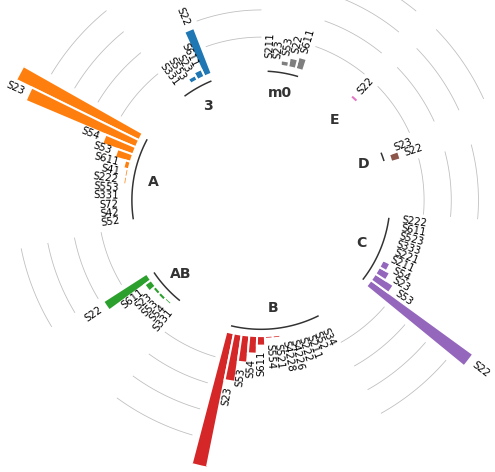
\includegraphics[width=12cm, height=11cm]{circular_barplot.png}
    \caption{Circular barplot pour la distribution hiérarchique du type de gloses utilisé par main.}
\end{figure}

Il devient évident qu'une certaine typologie est privilégiée par toutes les mains, y contribuant à des taux différents, en tenant toujours compte de la quantité de gloses que chaque main a écrites. \\


\begin{itemize}
    \item  \fbox{S22} Synonyme ;
    \item  \fbox{S23} Définition ;
    \item   \fbox{S53} Précisions sur le texte, glose élucidant le sens ;
    \item   \fbox{S54} Étymologie ;
    \item   \fbox{S611} Correction critique du texte (y compris des ajouts postérieurs).
\end{itemize}

Un tableau complet se trouve ci-dessous : 
\begin{figure}[H]
    \begin{subfigure}{0.40\textwidth}
    \centering
    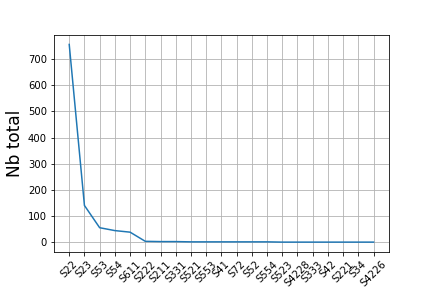
\includegraphics[width=9cm]{typologie_privilegiee.png}
    \caption{Typologies privilegiées }
    \end{subfigure}
    \begin{subfigure}{0,40\linewidth}
    \centering
    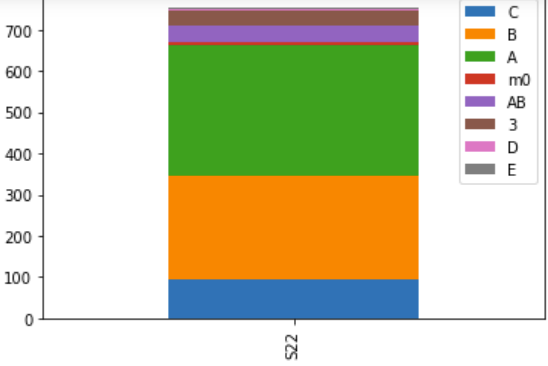
\includegraphics[width=7cm]{S22.png}
    \caption{Synonyme}
    \end{subfigure}
    \begin{subfigure}{0,40\linewidth}
    \centering
    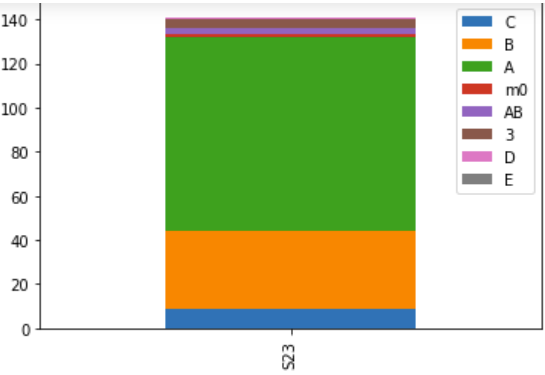
\includegraphics[width=7cm]{S23.png}
    \caption{Définition}
    \end{subfigure}
     \begin{subfigure}{0,40\linewidth}
    \centering
    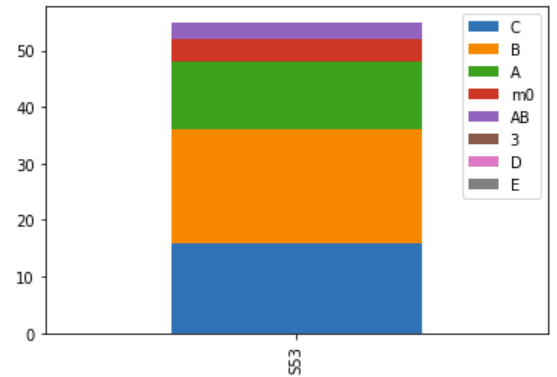
\includegraphics[width=7cm]{S53.png}
    \caption{Élucide les ambiguités du texte}
    \end{subfigure}
    \begin{subfigure}{0,40\linewidth}
    \centering
    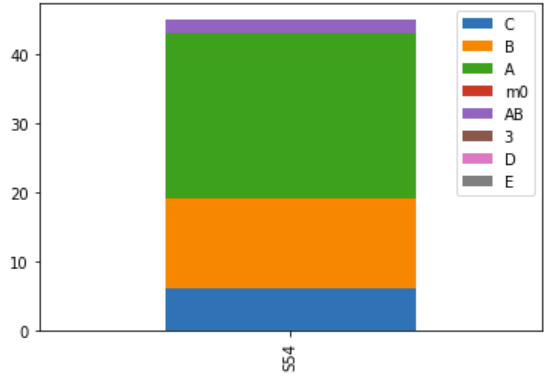
\includegraphics[width=7cm]{S54.png}
    \caption{Étymologie}
    \end{subfigure}
        \begin{subfigure}{0,80\linewidth}
    \centering
    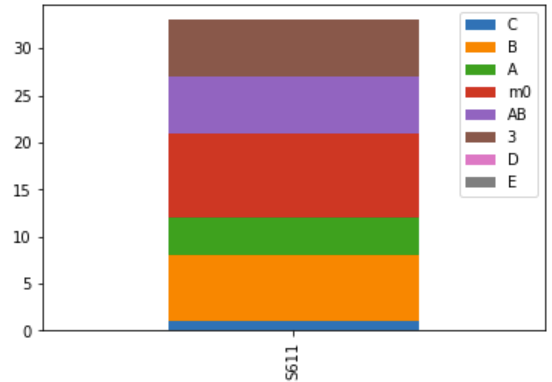
\includegraphics[width=7cm]{S611.png}
    \caption{Intervention éditoriale : corrections}
    \end{subfigure}
\end{figure} 

\clearpage

Outre les tendances générales, qui constituent les cas de base lors d'une annotation, ce sont les typologies moins fréquentes qui font la différence dans le caractère d'une campagne d'annotation ou le \og{} style \fg{} d'un glosateur. Plus précisement:

Pour A:

\begin{itemize}
    \item \fbox{S41} Signe de construction syntaxique (2 occurences)
    \item \fbox{S42} Mot(s) explicitant la construction (1 occurence)
\end{itemize}

Pour B:

\begin{itemize}
    \item \fbox{S554} Commentaire mythologique (2 occurences)
    \item \fbox{S521} \og{} quia\fg{} gloses (2 occurences)
    \item \fbox{S34} Indication d'adverbe (1 occurence)
    \item \fbox{S4226} supplétive par un adverbe (1 occurence)
    \item \fbox{S4228} supplétive par un verbe (1 occurence)
\end{itemize}

Pour C:

\begin{itemize}
    \item \fbox{S333} morphologie du \textit{modus} (2 occurences)
    \item \fbox{S221} négation d'un antonyme (1 occurence)
\end{itemize}

Si peu nombreuses que ce soient ces occurences, les groupes concernés, grâce à leur spécificité, permettent de déterminer un certain nombre de caractéristiques, relatives soit à la collection, soit aux préoccupations personnelles de chaque glosateur. Ainsi, entre autres, la main A se soucie assez spécifiquement de la construction syntaxique des lemmes qu'elle glose. Il en va de même pour la main C et les explications sur le \textit{modus} du verbe, ou pour la main B et son souci sur les adverbes. Ces typologies appartiennent plutôt à la sphère de l'explication grammaticale et révèlent les objectifs pédagogiques. Ces gloses sont potentiellement le produit original de chaque glosateur, plutôt qu'une copie directe de l'\textit{exemplar}, et ne renseignent que peu sur la \textit{recensio} du texte.\\

Il n'en va pas de même pour les typologies S554,S521 et S221. Un commentaire mythologique -ici pour les lemmes \textit{cupido}(quidam deus) et \textit{flamen} (sacerdotum iouis significat)- peut être originaire d'une collection ou source spécifique, comme un glossaire. Pareillement pour les \og{}quia-gloses\fg{}, un commentaire explicatif introduit par \textit{quia}(=parce que), et pour la négation d'un antonyme, qui n'apparaît pas aussi souvent que le synonyme exact d'un lemme. Encore, une comparaison entre temoins peut élucider le taux  d'originalité et le \og{}poids\fg{} qu'on attribuera à chaque glose\footnote{classification tirée de : \cite{steinova2021glosses},Introduction} .\\

Le poids d'une glose reflète sa (non-)trivialité :

\begin{itemize}
\item w=1 : une glose très triviale, qui aurait pu être et a probablement été inventée plusieurs fois indépendamment (par exemple, complète une ellipse dans une phrase) ;
\item w=2 : glose moins triviale, qui aurait pu être inventée plusieurs fois indépendamment, mais moins probable qu'une glose ayant le poids 1 ;
\item w=3 : glose non triviale, qui a peu de chances d'avoir été inventée plusieurs fois, mais dont l'apparition parmi les gloses partagées indique plutôt une transmission ;
\item w=4 : glose très peu triviale, qui ne peut être considérée comme ayant été inventée plusieurs fois et qui reflète donc clairement une véritable relation philologique.
\end{itemize}
Une fois que davantage de témoins ont été transcrits et qu'une collection parallèle de gloses a été établie, ces observations initiales se prêteront à une analyse plus fondée. Quoi qu'il en soit, cet exemple est révélateur de la manière auxiliaire dont une analyse exploratoire peut contribuer à une étude proche plus centrée, surtout lorsqu'il s'agit de données hétérogènes et à facettes multiples.

\chapter{Limites et perspectives}
\section{Un modèle de SegmOnt(ation)}

Certes, terminer la présentation d’un tel traitement ayant parcouru en détail tout aspects abordés est impossible. En effet, l’objectif même de cette recherche était d’ouvrir un dialogue. Par conséquent on note quelques points spécifiques embauchés qui nécessitent plus d’élaboration pour l'année prochaine.\\

En se penchant sur l'idée de la reconnaissance de texte plutôt que la reconnaissance des caractères\footnote{\url{http://www.bulac.fr/node/2491},p.83}, il reste en effet des enjeux, variables et spécifiques à un ensemble de documents, en particulier l’analyse de la mise en page et le sens de lecture de cette mise en page.Compte tenu de cette complexité des manuscrits glosés évoquée à plusieures reprises,  nous regrettons de ne pas disposer d'un modèle de segmentation qui identifierait principalement les lignes où réposent les gloses et les zones marginales où on trouve souvent des commentaires en \textit{catena}.Ceci étant dit, il est possible , une fois que davantage de données auront été collectées, de les combiner avec les modèles entraînés pour le projet \textit{Gallicorpora} et d'évaluer le résultats sur les témoins tels que lat.7499 (Figure. 3.1.). 

\begin{figure}[H]
    \centering
    \includegraphics[width=13cm, height=18cm]{miseenpage_commentaire_Rémi.png}
    \caption{La mise en page du BnF lat.7499 qui accueille en même temps le texte d'Eutychès, des gloses interlinéaires et le commentaire de Rémi d'Auxerre en marge. Les différentes couleurs marquent des Zones distinctes, les fleches le sens de lecture et les lignes noires l'intéraction entre les niveaux.}
\end{figure}

En même temps, Professeur Stokes lors d'un entretien sur le modèle de segmentation, m'a proposé une solution ingénieuse pour le marquage automatique des interlignes. En utilisant les polygons, présents dans l'élémént <Polygon> du fichier ALTO,il est possible de calculer la longueur des interlignes par rapport aux lignes principales, en soustrayant la longueur de l'interligne de celle de la ligne principale. Via un script pyhton et lxml, nous pouvons changer le TAGREFS en l'ID d'une ligne en question dans le fichier ALTO, chaque fois qu'elle mesure une certaine longueur - qui correspond à une InterlinearLine. Par exemple, au sein de la MainZone, si la ligne principale mésure \textbf{X} pixels, et la plus longue glose \textbf{x} pixels, toute ligne qui mésure \textbf{x} pixels ou moins est automatiquement marqué en tant qu'InterLinearLine. Cette méthode pourrait éventuellement être appliquée aux pages écrites uniquement en longues linges, car malheureusement la longueur des lignes à l'intérieur des colonnes coïncide forcement avec celle des gloses.

\section{Balisage automatique du couple lemme/glose}

Sans aucun doute, la partie la plus longue et la plus difficile de l'encodage a été de repérer, vérifier et baliser les couples lemmes-glosses. Etant donné les multiples attributs spécifiques et xml:id que chacun nécessite, le processus, afin d'obtenir la granularité fine souhaitée, est aussi chronofage que fastidieux. Franck Cinato\footnote{\cite{cinato2015priscien},p.211} a déjà constaté qu'un encodage assez fin et à double tranchant : \blockquote{Une telle approche se heurte à la limite imposée par la durée que réclame l’étape de marquage des types selon des codes informatiquement exploitables. Toutefois, la lourdeur du système se trouve compensé par l'utilité de l'intérogation.} \\

Parallèlement, un encodage manuel,(surtout quand on est confronté à la pression du temps et à un nombre élevé de gloses), est sujet aux \textit{lapsus} humains. A plusieurs reprises,la vérification de l'encodage et la correction des erreurs a rendu le processus encore plus long. En effet, afin d'assurer la qualité de nos données, nous avons dû itérer trois fois la même demarche en 1) notant dans un fichier excel toutes les informations concernant les gloses, 2) encodant ces informations 3) vérifiant l'encodage.Pour toutes ces raisons,et par souci de cohérence et de validité de nos données, un reperage automatique du couple lemme-glose devrait être mis en place.  Voici une solution proposée par Professeur Thibault Clérice que l'on peut appeler, vu son méchanisme, \textit{One Transcription Does it All} (OTD). La solution consiste à annoter manuellement les lemmes et leurs gloses correspondants dès la phase de transcription, que l'on peut ensuite transformerde plusieurs manières, comme indiqué le schéma ci-dessous (Figure 3.2.) : 

\begin{figure}[H]
    \centering
    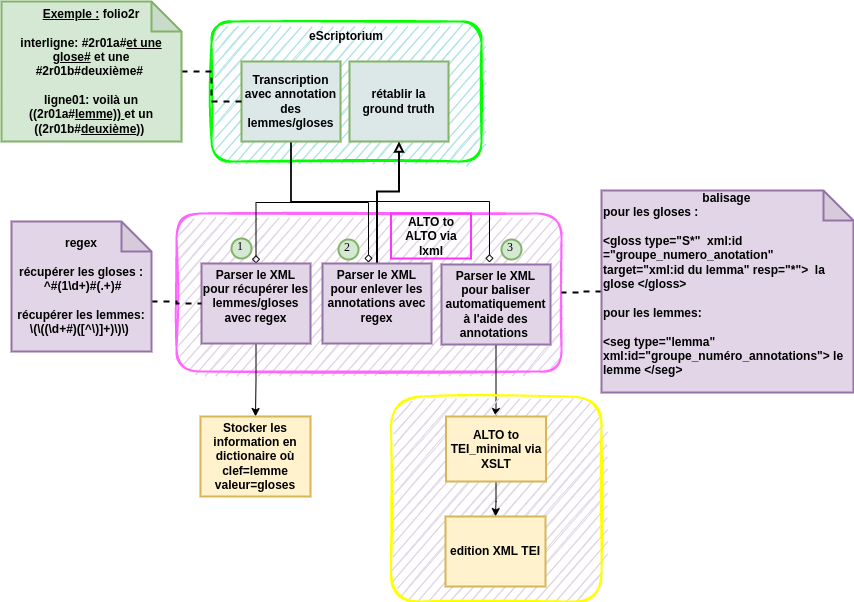
\includegraphics[width=14cm, height=10cm]{OTD.png}
    \caption{Modelisation de l'approche \textit{One Transcription Does it All}}
\end{figure}

Tout d'abord, un marquage manuel a lieu, qui consiste à entourer les lemmes et les gloses potentiels par une combinaison de signes (cf. Fig1.3. note en haut à droite) qui contient les coordonnées de chace element (page,ligne,ordre d'apparition dans la ligne). La deuxième étape,une fois les fichiers ALTO exportés, consiste en 3 opérations distinctes (d'où la polyvalence de la transcription initiale). En premier lieu (petite boule verte (1)), l'utilisation de regex permetra de capturer les groupes d'intérêt et de les stocker en forme d'un dictionnaire où \{clef = "lemme" : valeur= "glose"\}. En deuxième lieu (petite boule verte (3)), la même opération peut déboucher à un balisage automatique du couple lemme-glose, en substituant le marquage manuel par la balise souhaitée (cf. figure 3.1 au milieu à droite). Ainsi, la possibilité s'ouvre de créer la base d'un encodage XML-TEI via python et lxml (partie jaune). Troisième et dernière opération (petite boule verte (2)), le rétablissement de la vérité terrain qui est perturbée, via l'enlèvement du marquage initial. 

\begin{figure}[H]
    \centering
    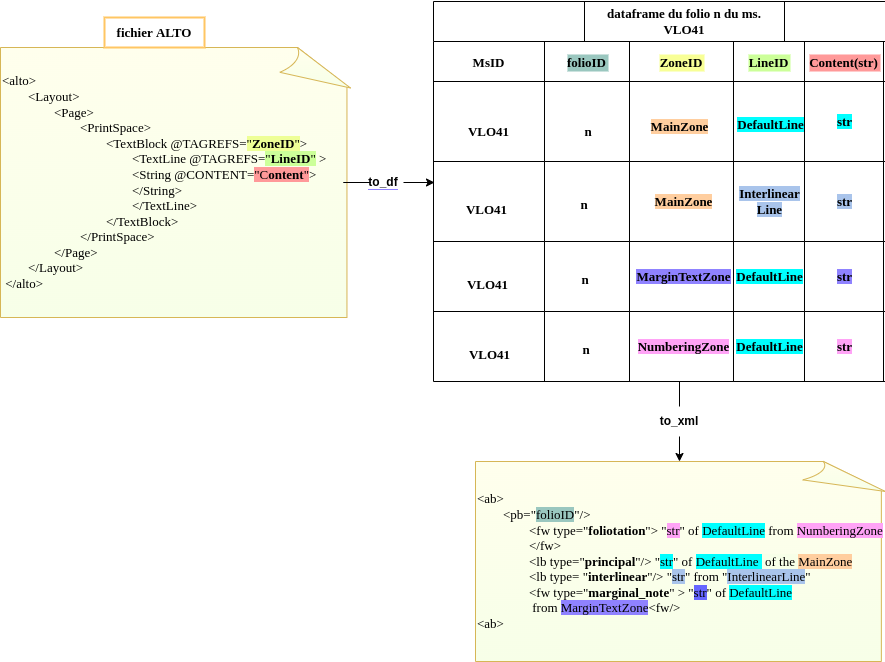
\includegraphics[width=14cm, height=11cm]{ALTO_to_df.drawio.png}
    \caption{Alternative : Stockage en dataframes et transformation via lxml }
\end{figure}

Une méthode alternative (Figure 3.2) qui peut complémenter la précédente a été portée à notre attention par Professeur Chahan Vidal-Gorène, qui vise au stockage et à la transformation des fichiers ALTO économiques et efficaces. Du fichier ALTO exporté, porteur de l'annotation SegmOnto, on passe à un dataframe qui classe le contenu par manuscrit, folio, type de zone et type de ligne concernée, tel que présenté dans la Figure 3.3.Cette méthode s'avère pratique pour la structuration et la comparaison des témoins par l'extraction des elements à exploiter. \\

Au moment où ce mémoire est en cours de rédaction, une option \og{} Annotations \fg{} est en cours d'implémentation dans eScriptorium ( pour l'instant toujours en phase beta), qui peut éventuellement donner une réponse définitive à cette question. Une fois implementée, elle permetra une annotation sémantique des morceaux de texte avec des étiquettes personnalisées, comme les lemmes et les gloses. A condition que ces étiquettes figurent dans le fichier exporté, cela devrait rendre le reperage des lemmes et gloses possible dès la phase de la transcription sans perturber la verité de terrain.


\section{Nouvelles perspectives - Portée du projet}

Enfin, il convient d'évoquer la portée que vise un tel projet sur la tradition manuscrite d'Eutychès, à savoir la réalisation de sa propre édition de gloses.
Comme il a déjà été évoqué maintes fois, le caractère fluide, non linéaire et polygénique des gloses et la nature complexe de leur transmission (non seulement par copie d'un exemplaire à un autre, mais aussi oralement et peut-être après avoir été longtemps conservées en mémoire) ne permettent pas une édition critique au sens traditionnel. Un cadre critique alternatif impose plutôt la présentation du matériel en tant que réseau, représentant les modalités du rapport et de la similarité entre les témoins. Sur ce cadre alternatif, Evina Steinova décrit le processus \footnote{\cite{steinova2021glosses}, Introduction, Network as a model for a Digital Scholarly Edition.}:

\blockquote{In this framework, several entities (manuscript witnesses, clusters of glosses transmitted together, and chapters of the first book of the Etymologiae) appear as nodes. Glosses that are common to multiple of these entities appear as edges that connect them. In this manner, the users of the edition can access the corpus from several different angles and simultaneously view it in its entirety and dissected into its many constituent entities (clusters, layers of glosses in particular witnesses, and individual glosses).}

Avant d'être en mésure de réaliser une édition numérique de ce type, plusieurs étapes doivent être réalisées, selon une méthodologie spécifique. Les témoins manuscrits, une fois que chaque signe a été transcrit et examiné, doivent être classés selon la typologie des gloses. En l'absence de datation précise de la copie des gloses, une typologie ne peut être réalisée qu'après avoir rassemblé des échantillons significatifs pour chacune d'entre elles. Les échantillons collectés devraient permettre d'identifier des couches de composition dans le contenu des gloses, et ainsi de définir des étapes dans le développement du corpus de gloses dans le Haut Moyen Âge. Ensuite, un manuscrit de base contenant une version étendue des gloses est choisi et les variantes du reste des manuscrits sont collationnées contre son texte. Le petit nombre de manuscrits glosés pour Eutychès permet de considérer l'ensemble du corpus.  Cette activité comparative permettra la création d'un thésaurus des gloses, chaque \og{}archétype\fg{} de glose - une glose au sens abstrait, instanciée dans différentes versions - recevant un identifiant xml:id unique. Ce n'est qu'alors que des réseaux de gloses pourront être projetés et que des conclusions pourront être déduites sur leur contenu, en fonction de la tradition manuscrite. 


\section{Conclusions générales}

L'objectif de cette étude était de démontrer, tout d'abord, au niveau théorique, l'intérêt que présente la tradition des manuscrits glosés du \textit{De uerbo} d'Eutychès, notamment sa mise-en-page particulière et ses différents niveaux d'annotaiton. Dans un deuxième temps, nous avons cherché à mettre en évidence les différentes moyens dont les outils numériques s'avèrent essentiels pour la description et la manipulation adéquates des documents d'une telle nature.Plusieurs technologies ont été appliquées à notre cas d'étude, allant de la reconnaissance automatique du texte jusqu'à l'encodage et à la lecture distante du corpus via la visualisation de ses composants.Au même moment, les limites et les moyens d'optimiser notre approche ont été évoqués. Ce qui reste à faire et que nous tâcherons à accomplir dans l'année qui vient, suppose tout d'abord une augmentation du jeu de données, en incluant plusieurs témoins et l'optimisation du pipeline, afin de le rendre aussi cohérent et automatique que possible, tout en veillant à la qualité et à l'interopérabilité des données concernées.


%Afficher bibliographie
\newpage
\nocite{*}
\printbibliography

% table des figures
\listoffigures

\end{document}
